\documentclass[fontsize=12pt, DIV=15, parskip=half-]{scrartcl}

\usepackage[utf8]{inputenc}
\usepackage[german]{babel}
\usepackage[T1]{fontenc}
\usepackage{lmodern}
\usepackage[lf]{libertine}
\usepackage{pgfpages}
\usepackage{tikz}
\usepackage{textcomp}
\usepackage{microtype}
\usepackage{array}
\usepackage[inline]{enumitem}
\usepackage[intlimits]{amsmath}
\usepackage{amssymb}
\usepackage{amsfonts}
\usepackage[amsmath, thmmarks]{ntheorem}
\usepackage[italic, defaultmathsizes, basic]{mathastext}
\usepackage{mathtools}
\usepackage{stmaryrd}
\usepackage{booktabs}
\usepackage{nicefrac}
\usepackage{ifthen}
\usepackage{suffix}
\usepackage{cancel}
\usepackage{setspace}
\usepackage{stmaryrd}
\usepackage{hyperref}
\usepackage{nameref}

\linespread{1.05}

\theoremstyle{break}
\theoremheaderfont{\sffamily\bfseries}
\theorembodyfont{\upshape}
\newtheorem{aufgabe}{Aufgabe}
\newtheorem{loesung}{Lösung zu Aufgabe}
\newtheorem{ergaufgabe}[aufgabe]{$^*$Aufgabe}
\newtheorem{ergloesung}[loesung]{Lösung zu Aufgabe}

\newcommand{\defin}[1]{\textbf{\textit{\color{blue}#1}}}
\newcommand{\anm}[1]{~~\hfill(#1)}
\newcommand{\defanm}[1]{~~\hfill\defin{(#1)}}
\newcommand{\N}{\mathbb{N}}
\newcommand{\Z}{\mathbb{Z}}
\newcommand{\Q}{\mathbb{Q}}
\newcommand{\R}{\mathbb{R}}
\newcommand{\C}{\mathbb{C}}
%\newcommand{\cal}[1]{\mathcal{#1}}
\newcommand{\tmenge}[2]{\smash{\{#1\mathbin|#2\}}}
\newcommand{\menge}[2]{\left\{#1\:\middle|\:#2\right\}}
\newcommand{\rk}[1]{\left(#1\right)}
\newcommand{\ro}[1]{\left[#1\right)}
\newcommand{\lo}[1]{\left(#1\right]}
\newcommand{\ab}[1]{\left[#1\right]}
\newcommand{\st}[1]{\stackrel{\text{#1}}}
\newcommand{\stm}[1]{\stackrel{#1}}
\newcommand{\imp}{\Rightarrow}
\newcommand{\timp}[1]{\overset{\text{#1}}{\imp}}
\newcommand{\kimp}[1]{\overset{\mathclap{\text{#1}}}{\imp}}
\newcommand{\aeq}{\Leftrightarrow}
\newcommand{\ait}{\quad\aeq\quad}
\newcommand{\stait}[1]{\quad\stackrel{#1}\aeq\quad}
\newcommand{\ohne}[1]{\setminus \{#1\}}
\newcommand{\tim}[1]{\text{\quad #1 \quad}}
\newcommand{\taeq}[1]{\overset{\text{#1}}{\aeq}}
\newcommand{\kaeq}[1]{\overset{\mathclap{\text{#1}}}{\aeq}}
\newcommand{\tg}[1]{\overset{\text{#1}}{=}}
\newcommand{\kg}[1]{\overset{\mathclap{\text{#1}}}{=}}
\newcommand{\eps}{\varepsilon}
\renewcommand{\phi}{\varphi}
\renewcommand{\rho}{\varrho}
\newcommand{\CCC}{\operatorname{C}}
\newcommand{\DDD}{\operatorname{D}}
\newcommand{\MMM}{\operatorname{M}}
\newcommand{\Pot}{\mathfrak{P}}
\newcommand{\id}{\mathrm{id}}
\renewcommand{\leq}{\leqslant}
\renewcommand{\geq}{\geqslant}
\newcommand{\eee}{\mathrm{e}}
\newcommand{\iii}{\mathrm{i}}
\newcommand{\modu}{~\mathrm{modulo}}
\newcommand{\dd}[1]{\:\mathrm{d}#1}
\newcommand{\dt}{\dd{t}}
\newcommand{\dx}{\dd{x}}
\newcommand{\dxyz}{\dd{(x, y, z)}}
\renewcommand{\Re}{\operatorname{Re}}
\renewcommand{\Im}{\operatorname{Im}}
\newcommand{\Grad}{\operatorname{Grad}}
\newcommand{\Kern}{\operatorname{Kern}}
\newcommand{\Bild}{\operatorname{Bild}}
\newcommand{\Hess}{\operatorname{Hess}}
\newcommand{\tbetr}[1]{\mathopen|\smash{#1}\mathclose|}
\newcommand{\betr}[1]{\left|#1\right|}
\newcommand{\mmn}[2]{\begin{pmatrix} #1 \\ #2 \end{pmatrix}}
\newcommand{\tmmn}[2]{\smash{(\begin{smallmatrix} #1 \\ #2 \end{smallmatrix})}}
\newcommand{\mmmn}[3]{\begin{pmatrix} #1 \\ #2 \\ #3 \end{pmatrix}}
\newcommand{\mmnn}[4]{\begin{pmatrix} #1 & #2 \\ #3 & #4 \end{pmatrix}}
\newcommand{\mnnnn}[4]{\begin{pmatrix} #1 & #2 & #3 & #4 \end{pmatrix}}
\newcommand{\mmmmn}[4]{\begin{pmatrix} #1 \\ #2 \\ #3 \\ #4 \end{pmatrix}}
\newcommand{\mmmnnn}[9]{\begin{pmatrix} #1 & #2 & #3\\ #4 & #5 & #6\\ #7 & #8 & #9 \end{pmatrix}}
\newcommand{\mmmnn}[6]{\begin{pmatrix} #1 & #2 \\ #3 & #4\\ #5 & #6 \end{pmatrix}}
\newcommand{\mmnnn}[6]{\begin{pmatrix} #1 & #2 & #3\\ #4 & #5 & #6 \end{pmatrix}}

\newenvironment{mathex}[1][LLLLLLLLLLLL]{
  \[%
  \newcolumntype{L}{>{\displaystyle\setlength{\arraycolsep}{4pt}}l}%
  \newcolumntype{C}{>{\displaystyle\setlength{\arraycolsep}{4pt}}c}%
  \newcolumntype{R}{>{\displaystyle\setlength{\arraycolsep}{4pt}}r}%
  \setlength{\arraycolsep}{1.5pt}%
  \begin{array}{>{\vspace*{1.3ex}}#1}%
}{
  \end{array}%
  \vspace*{-1.3ex}%
  \]%
  \ignorespacesafterend%
}

\newcommand{\sternitem}{\refstepcounter{enumi}\item[($^*$\alph{enumi})]}

\newcounter{paeckchenteil}
\newcounter{paeckcheninzeile}
\newenvironment{paeckchen}[1][3]{
\setcounter{paeckchenteil}{0}
\setcounter{paeckcheninzeile}{0}
\renewcommand{\item}{%
\ifthenelse{\value{paeckchenteil}=0}{}{&}%
\ifthenelse{\value{paeckchenteil}>0 \and \value{paeckcheninzeile}=0}{\\}{}%
\refstepcounter{paeckchenteil}%
\stepcounter{paeckcheninzeile}%
\ifthenelse{\value{paeckcheninzeile}=#1}{\setcounter{paeckcheninzeile}{0}}{}%
\text{(\alph{paeckchenteil})}%
&
}%
\WithSuffix\newcommand\item*{%
\ifthenelse{\value{paeckchenteil}=0}{}{&}%
\ifthenelse{\value{paeckchenteil}>0 \and \value{paeckcheninzeile}=0}{\\}{}%
\refstepcounter{paeckchenteil}%
\stepcounter{paeckcheninzeile}%
\ifthenelse{\value{paeckcheninzeile}=#1}{\setcounter{paeckcheninzeile}{0}}{}%
\text{($^*$\alph{paeckchenteil})}%
&
}%
\renewcommand{\sternitem}{\item*}
\begin{mathex}[R>{\;\;}L>{\qquad}R>{\;\;}L>{\qquad}R>{\;\;}L>{\qquad}R>{\;\;}L>{\qquad}R>{\;\;}L>{\qquad}R>{\;\;}L>{\qquad}R>{\;\;}L]
}{
\end{mathex}
}

%\pagestyle{empty}
\begin{document}
\begin{center}
\Large\bfseries\sffamily JavaCrypTool (\url{www.cryptool.org})

Online-Hilfe zur Bedienung der Fleißner-Schablone  \\[0.1\baselineskip]
\normalsize\normalfont 
\end{center}
\vspace*{0.5\baselineskip}


\tableofcontents
\newpage

Die Hauptfunktion dieses Plug-ins ist die Analyse eines Geheimtextes, der durch die Fleißner-Schablone verschlüsselt wurde. Als Schlüssel gilt der Inhalt der Schablone. Etwas unüblich als Schlüssellänge bezeichnet man dabei die Seitenlänge des quadratischen Feldes (Schablone).

Neben der Analysefunktion stehen in diesem Plug-in auch die Funktionen \hyperlink{verschl}{Verschlüsselung} und \hyperlink{entschl}{Entschlüsselung} zur Verfügung.


\section{Analyse}
In der Ausgangseinstellung des Plug-ins (Default-Einstellung) sitzt der Radiobutton bei der Analysefunktion: Sie ist in der ersten Gruppierung \glqq Methode\grqq{}
ausgewählt. Hier kann die Methode auch auf die Verschlüsselung oder Entschlüsselung geändert werden.

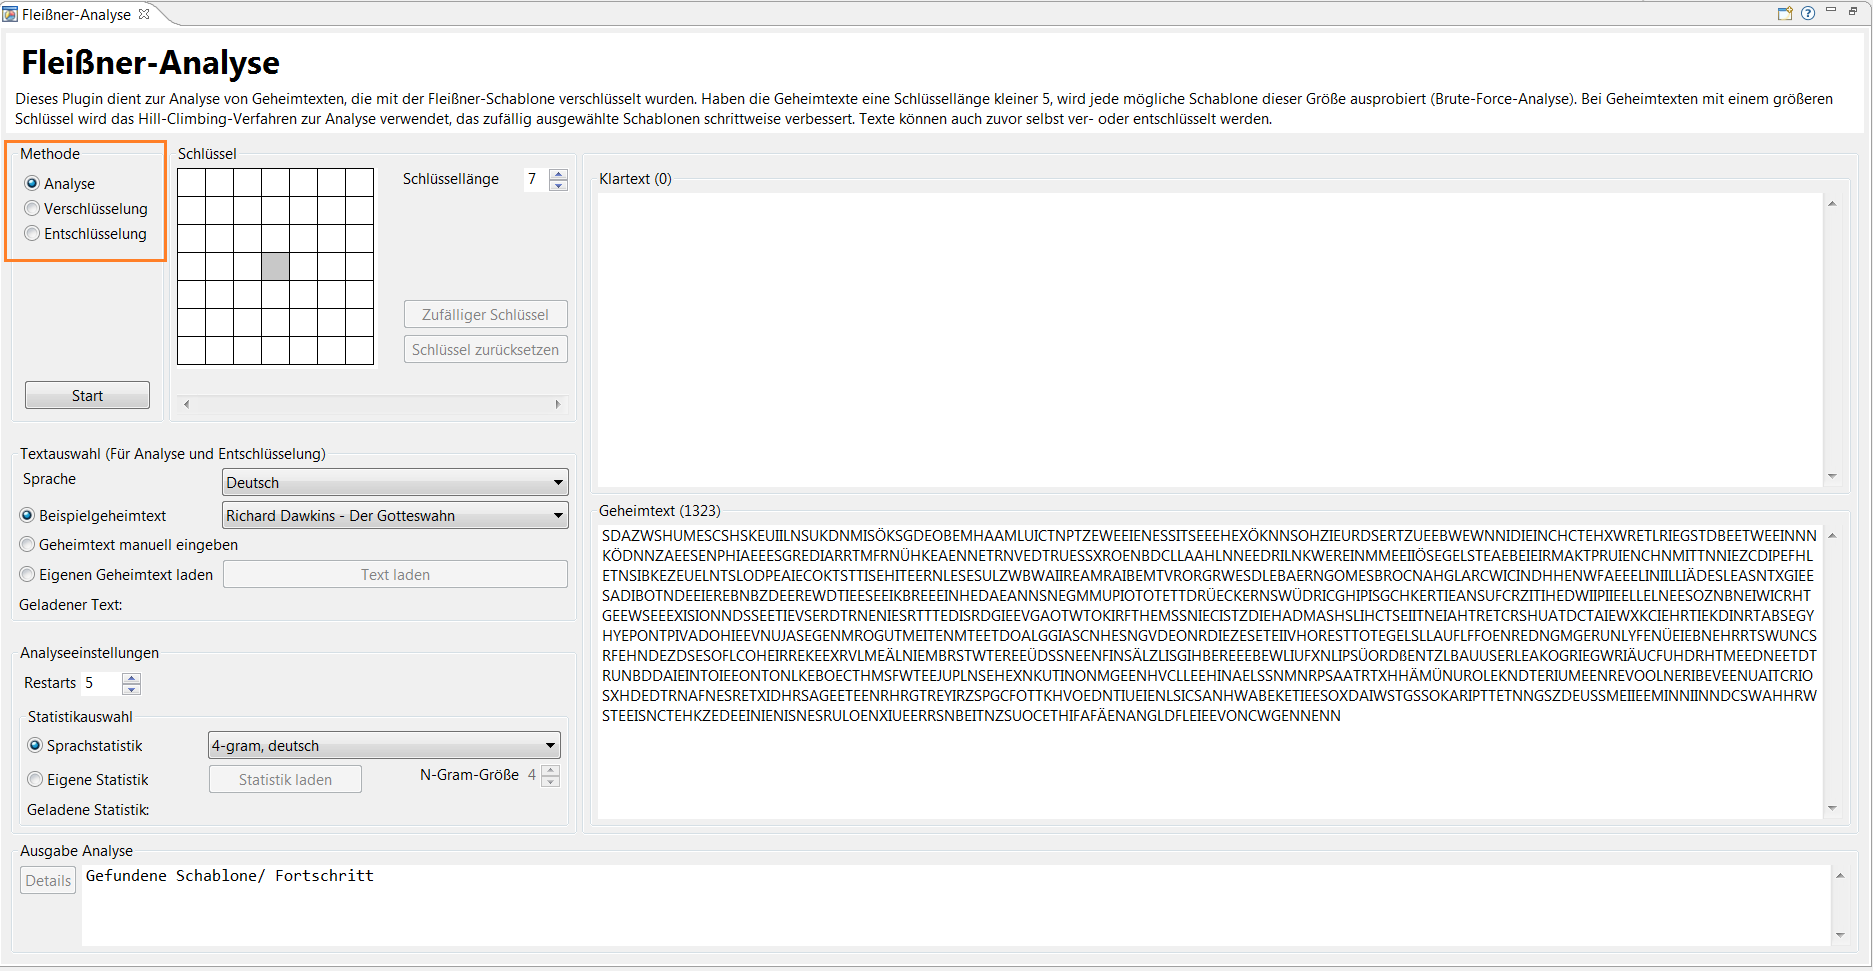
\includegraphics[scale=0.45]{FleissnerMethods.png}
%\newpage

Da beim Start des Plug-ins Vorgabewerte auch für den Geheimtext gesetzt werden, kann die Analyse durch die Betätigung des \glqq Start\grqq{}-Buttons direkt ausgeführt werden. 

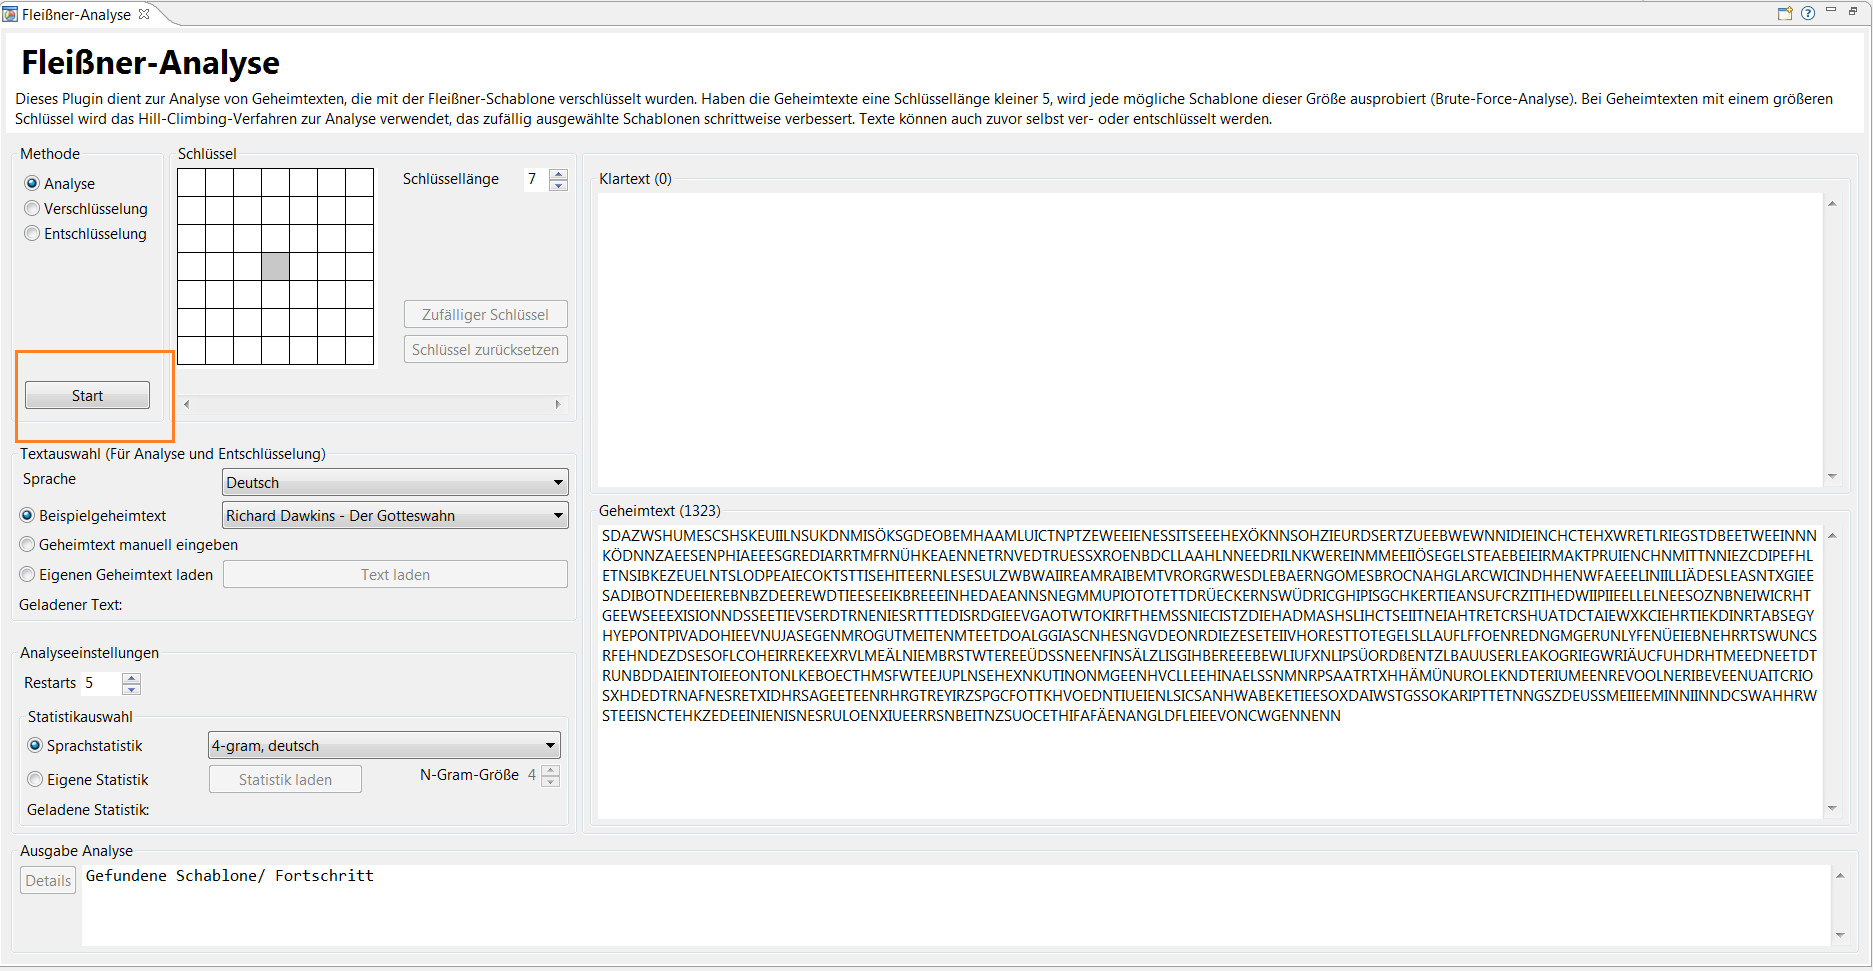
\includegraphics[scale=0.45]{FleissnerStart.png}
%\newpage

\subsection{Schlüssellänge}
Da der genutzte Schlüssel für die Analyse in der Regel geheim ist und erst gefunden werden soll, ist das Schlüsselfeld selbst bei dieser Funktionsauswahl deaktiviert. Die Schlüssellänge kann aber gewählt werden und sollte mit der des, für diesen Geheimtext verwendeten, Schlüssels übereinstimmen.

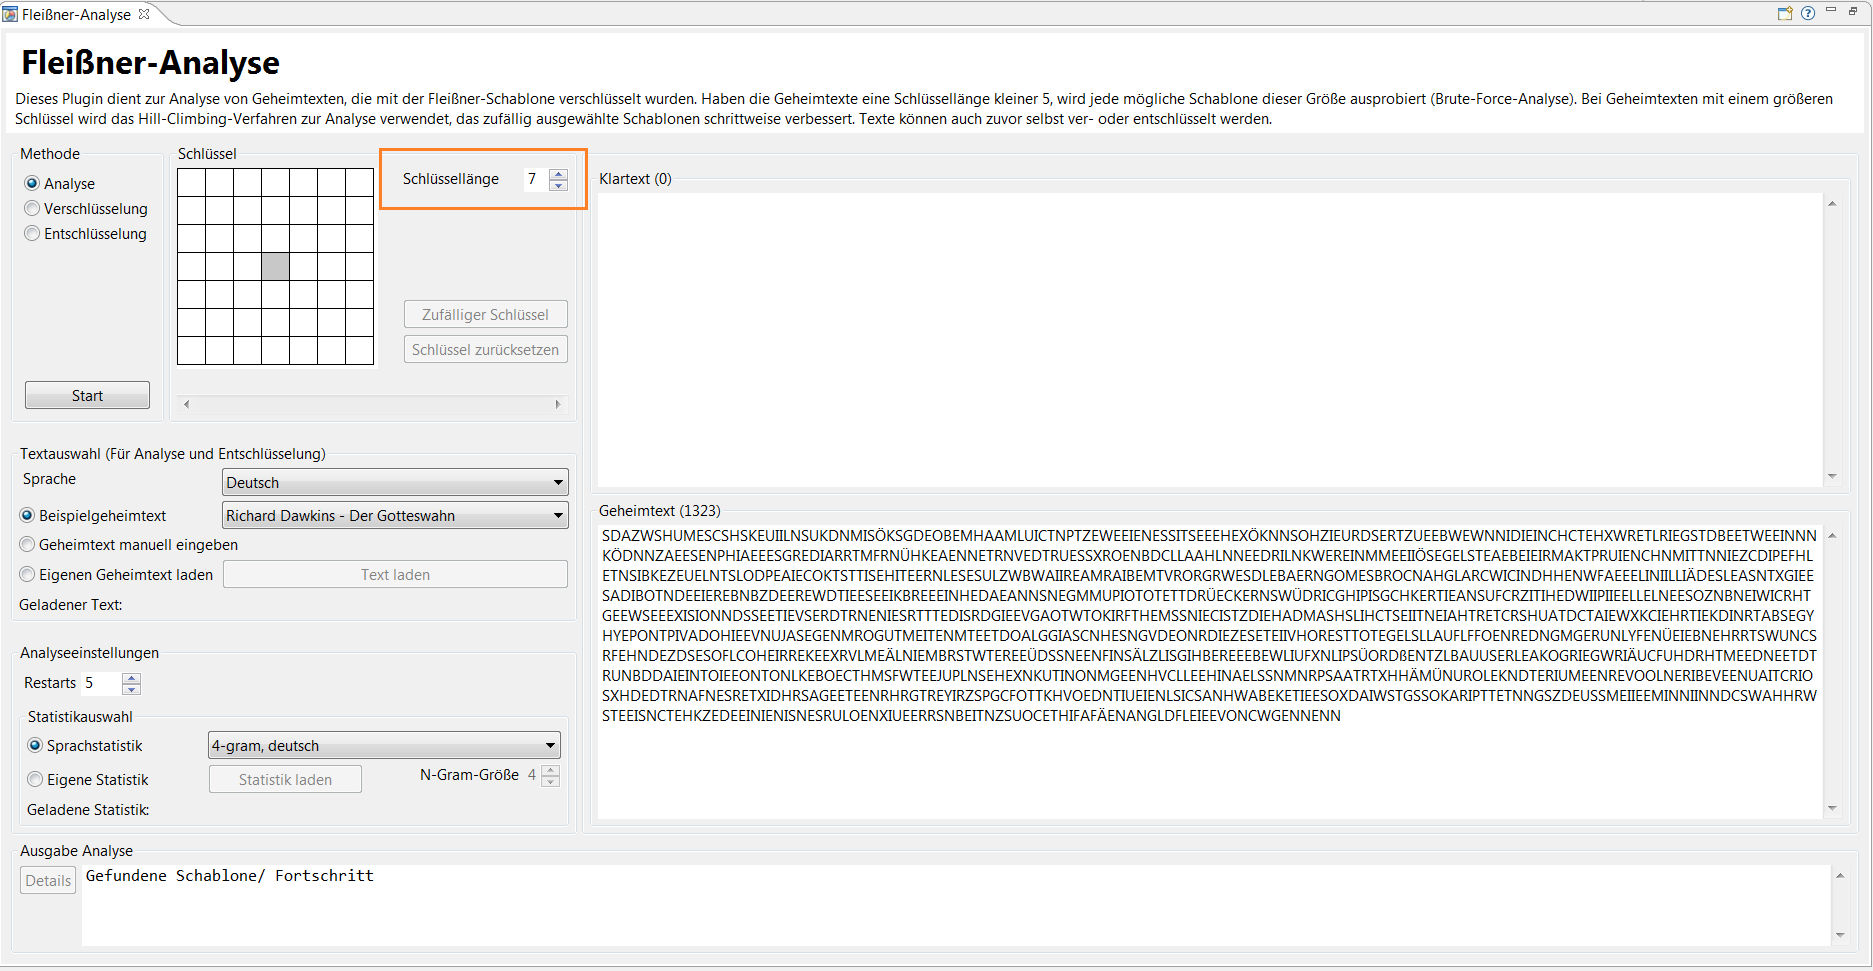
\includegraphics[scale=0.45]{FleissnerKeySize.png}


Ist bei der \hyperlink{txtausw}{Textauswahl}  \glqq Beispielgeheimtext\grqq{} (Voreinstellung) ausgewählt, so wird der Geheimtext der jeweiligen Schlüssellänge angepasst. Der dazu verwendete Schlüssel wird zufällig erzeugt und nach der Verschlüsselung wieder verworfen.

\subsection{Textauswahl} \hypertarget{txtausw}{}
\subsubsection{Sprache}
In dieser Gruppierung kann zwischen den Sprachen \glqq Deutsch\grqq{} und \glqq Englisch\grqq{} gewählt werden. Ist im Abschnitt \hyperlink{txteing}{Texteingabe} \glqq Beispielgeheimtext\grqq{} ausgewählt, so wird der angezeigte Text entsprechend der ausgewählten Sprache aktualisiert. 

Für einen manuell eingegebenen oder geladenen Geheimtext, muss die Sprache manuell ausgewählt werden. Der zu analysierende Text muss der hier ausgewählten Sprache entsprechen, da die Analyse auf sprachspezifischen Auftrittswahrscheinlichkeiten von Buchstabenketten beruht.

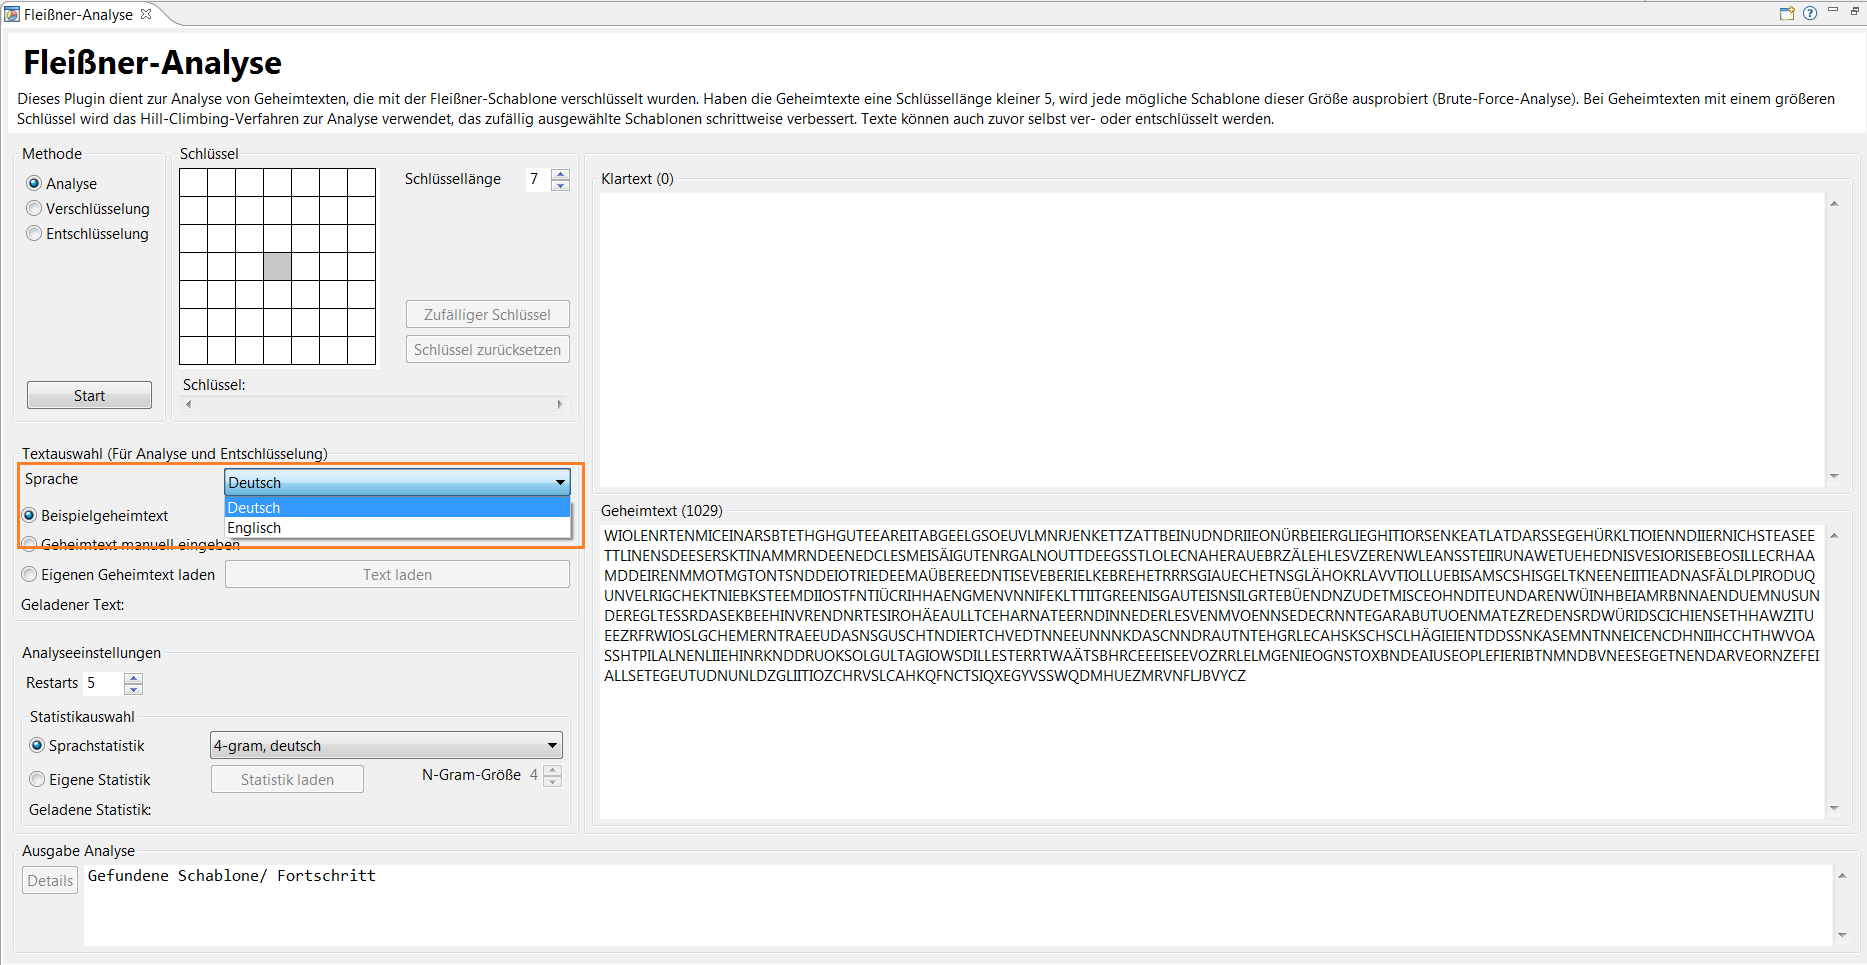
\includegraphics[scale=0.45]{FleissnerLanguage.png}
\newpage

\subsubsection{Texteingabe}\hypertarget{txteing}{}
In dieser Gruppierung kann die Art der Eingabe des Geheimtextes ausgewählt werden.

\begin{enumerate}[label=(\alph*), leftmargin=*]
\item \textbf{Beispielgeheimtext}

Voreingestellt ist hier die Auswahl \glqq Beispielgeheimtext\grqq. 
%\newpage
Hier kann zwischen zwei deutschsprachigen und zwei englischsprachigen
Geheimtexten gewählt werden. \footnote{\textbf{Quellen:}\\ Richard Dawkins - Der Gotteswahn\\ Richard Dawkins - The God Delusion\\ \url{https://de.wikipedia.org/wiki/Bildende_Kunst\#Fr\%C3\%BChchristliche_und_byzantinische_Kunst}\\ \url{https://en.wikipedia.org/wiki/Visual_arts}} 

Die Texte werden je nach ausgewählter Schlüssellänge entsprechend verschlüsselt. 

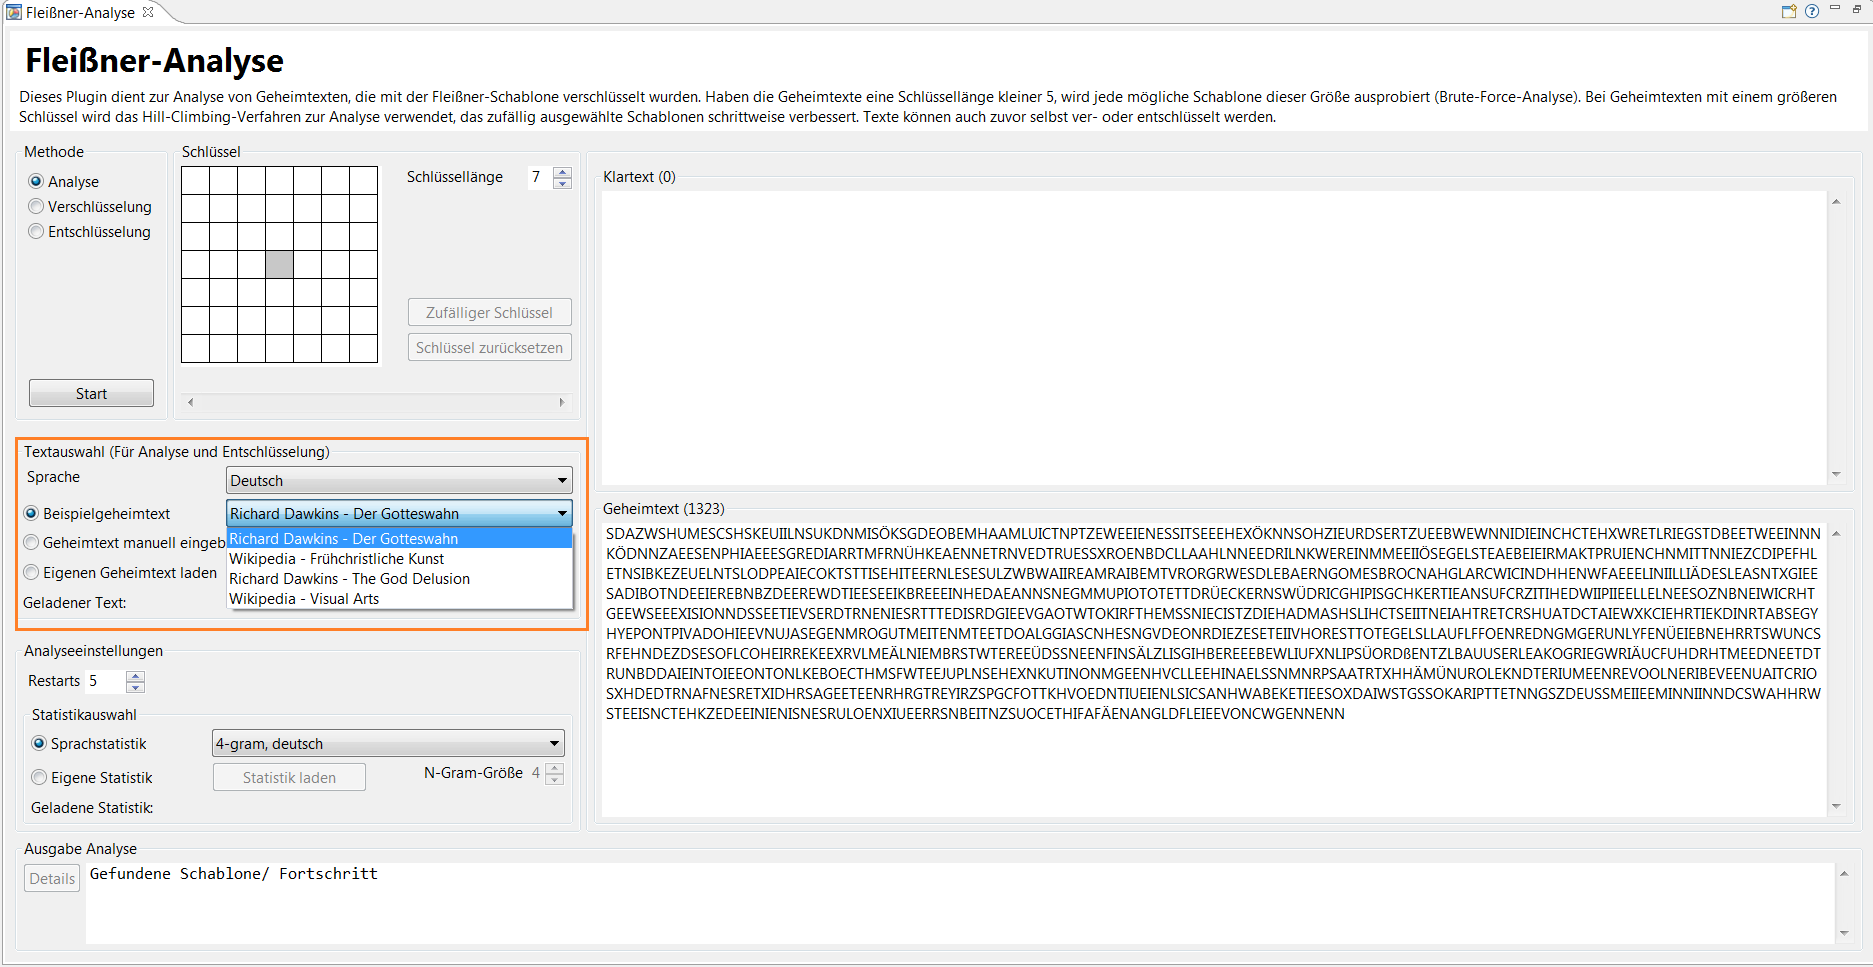
\includegraphics[scale=0.4]{FleissnerTxtAuswahl.png}
\newpage

\item \textbf{Geheimtext manuell eingeben}

Bei der Auswahl von \glqq Geheimtext manuell eingeben\grqq{} wird das Feld für den Geheimtext für die manuelle Eingabe freigeschaltet und es kann ein Text eingetippt werden.

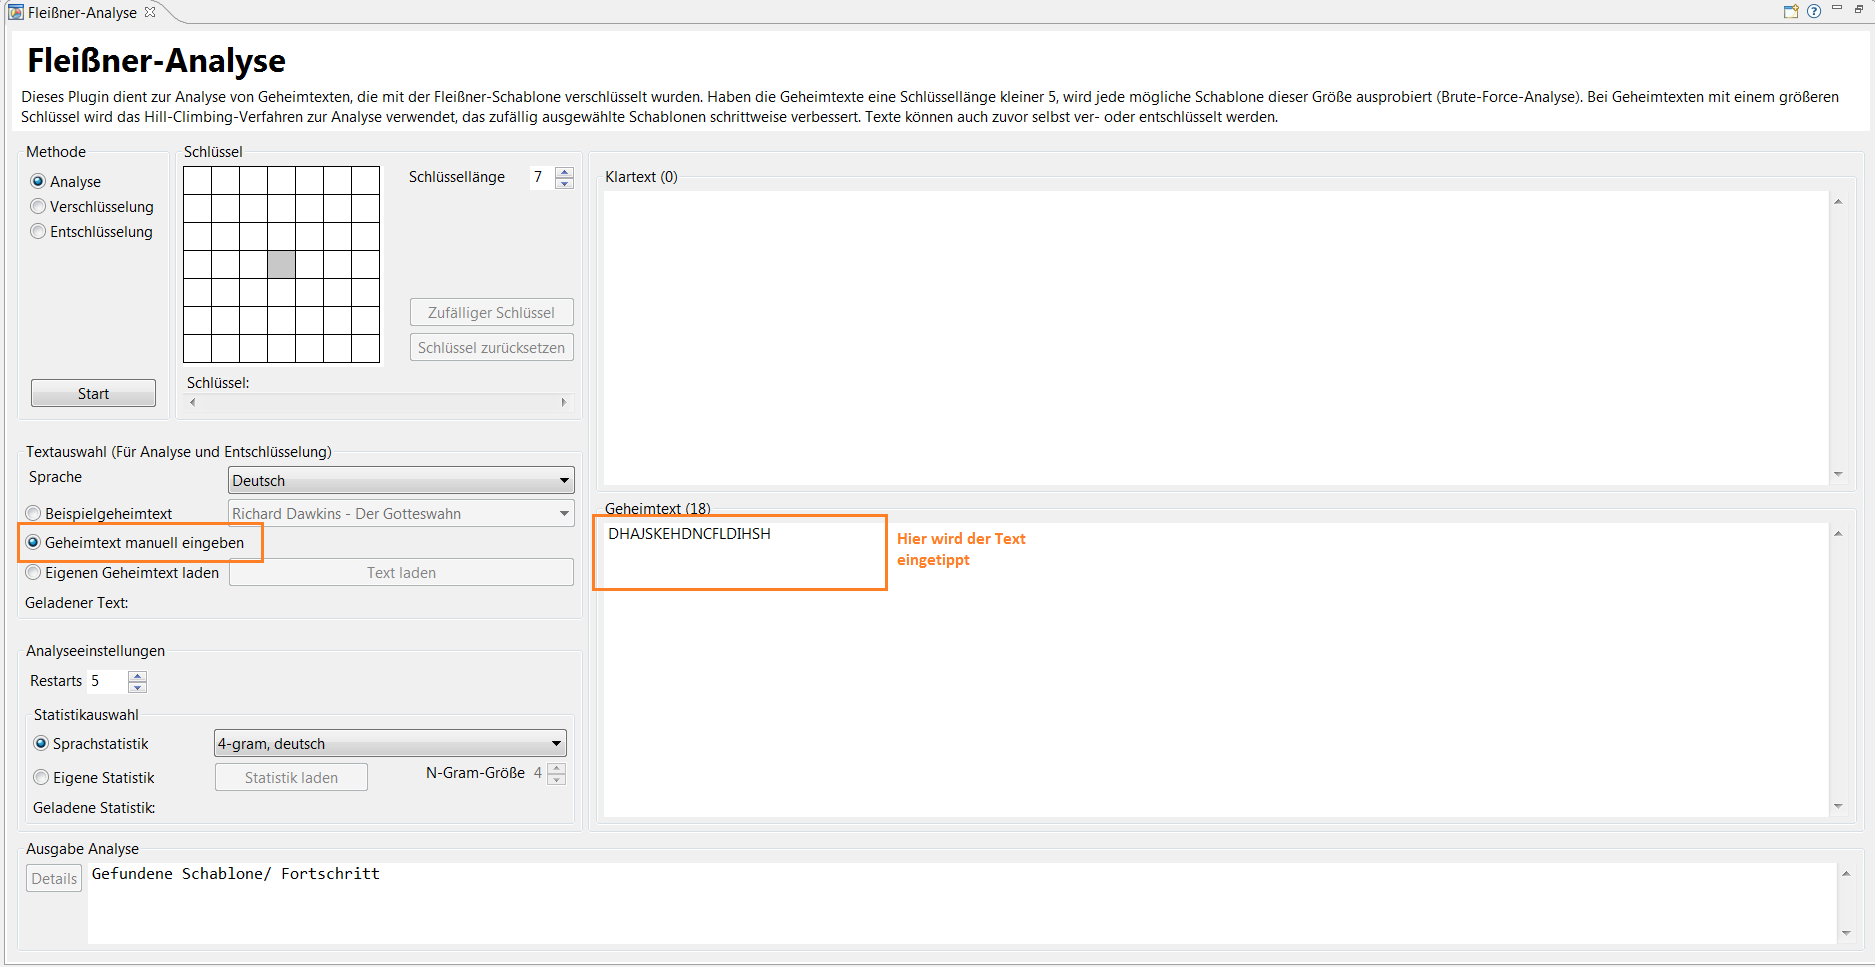
\includegraphics[scale=0.4]{FleissnerManGhtxt.png}

\item \textbf{Eigenen Geheimtext laden}

Zum Laden eines Geheimtextes aus einer Datei dient die letzte Auswahl \glqq Eigenen Geheimtext laden\grqq.
Bei dieser Auswahl wird der Button \glqq Text laden\grqq{} aktiviert, über den dann eine Textdatei (*.txt) geladen werden kann. Der Text wird dann im Geheimtextfeld angezeigt.

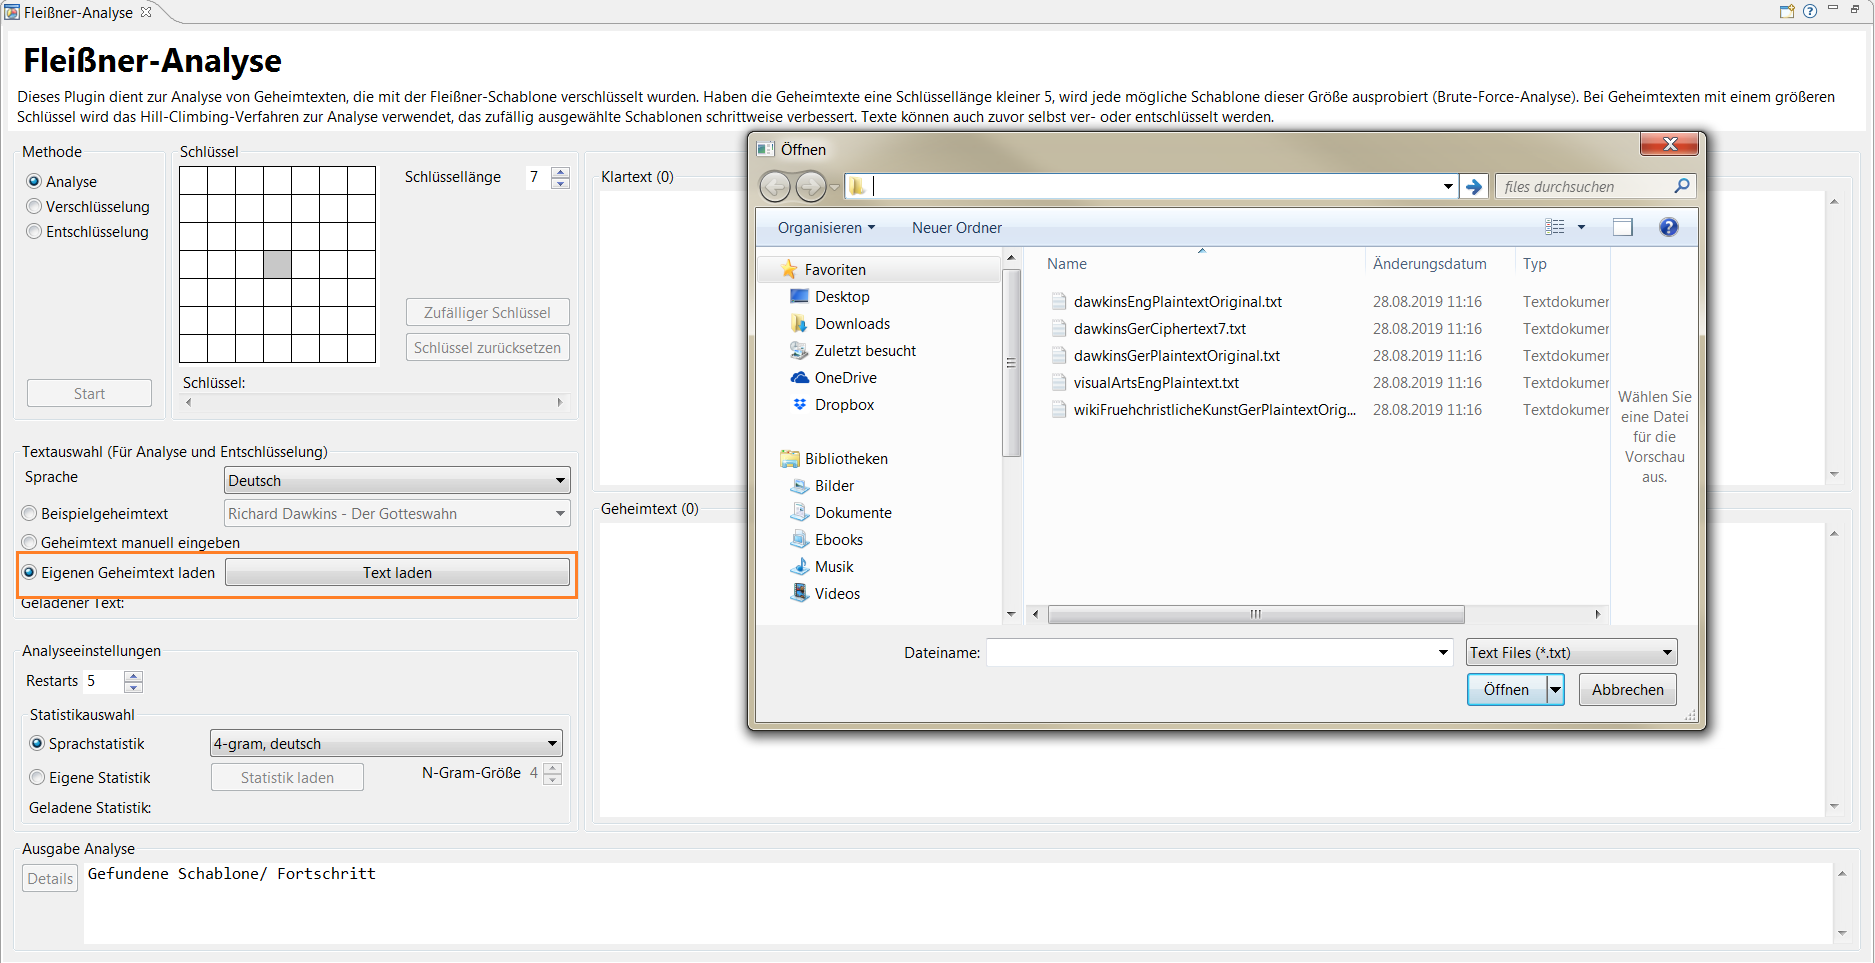
\includegraphics[scale=0.4]{FleissnerCipherLoadOwn.png}
\end{enumerate} 


\subsection{Analyseeinstellungen}
Die Gruppierung \glqq Analyseeinstellungen\grqq{} befindet sich direkt unter der Gruppierung \glqq\hyperlink{txtausw}{Textauswahl}\grqq{} und ist nur für die Analysefunktion aktiviert.

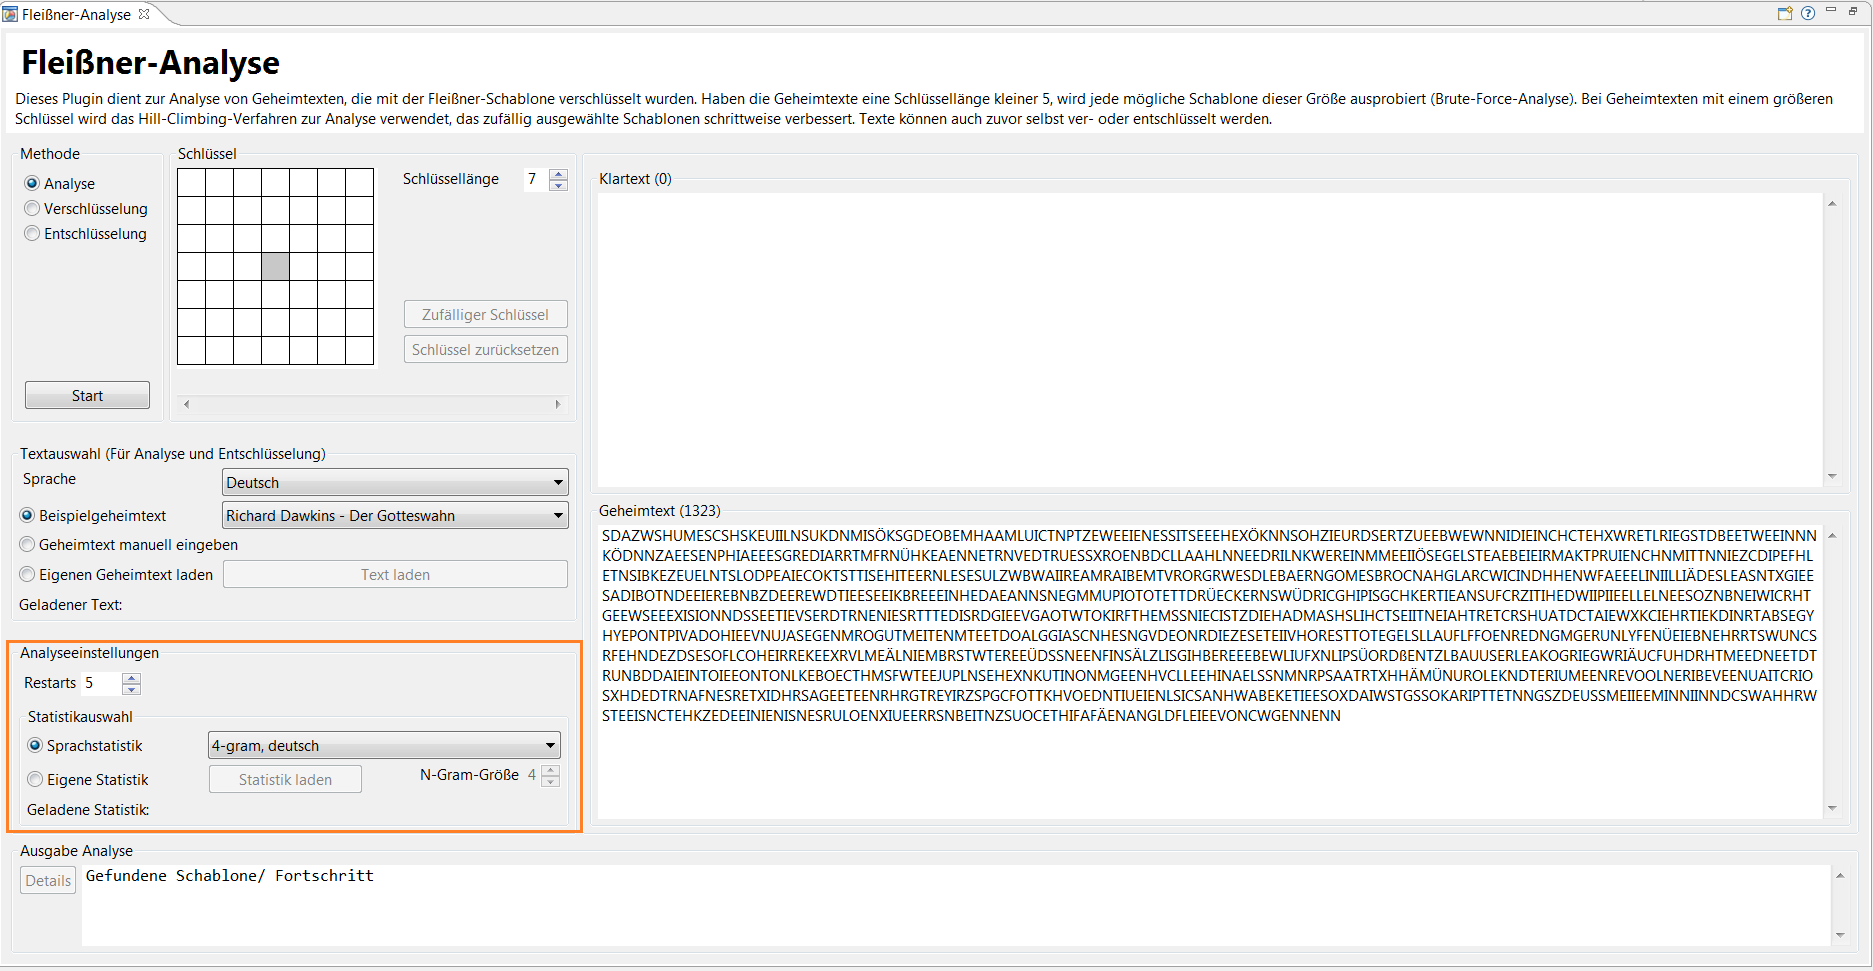
\includegraphics[scale=0.45]{FleissnerAnalysisSettings.png}


\subsubsection{Restarts}
Die Anzahl der Restarts ist relevant für die Analyse von Geheimtexten, die mit Schlüsseln der Größe 5 oder höher verschlüsselt wurden. Bei diesen Schlüsselgrößen wird das \glqq Hill-Climbing\grqq -Verfahren zur Analyse verwendet. Für jeden Restart wird zufällig eine Schablone in der gewählten Schlüssellänge erstellt. Diese Schablone wird dann schrittweise verändert, bis kein besserer Klartext durch die veränderte Schablone erzeugt werden kann. Je höher die Anzahl der Restarts, desto höher ist die Wahrscheinlichkeit, dass der richtige Schlüssel durch die Analyse gefunden wird.
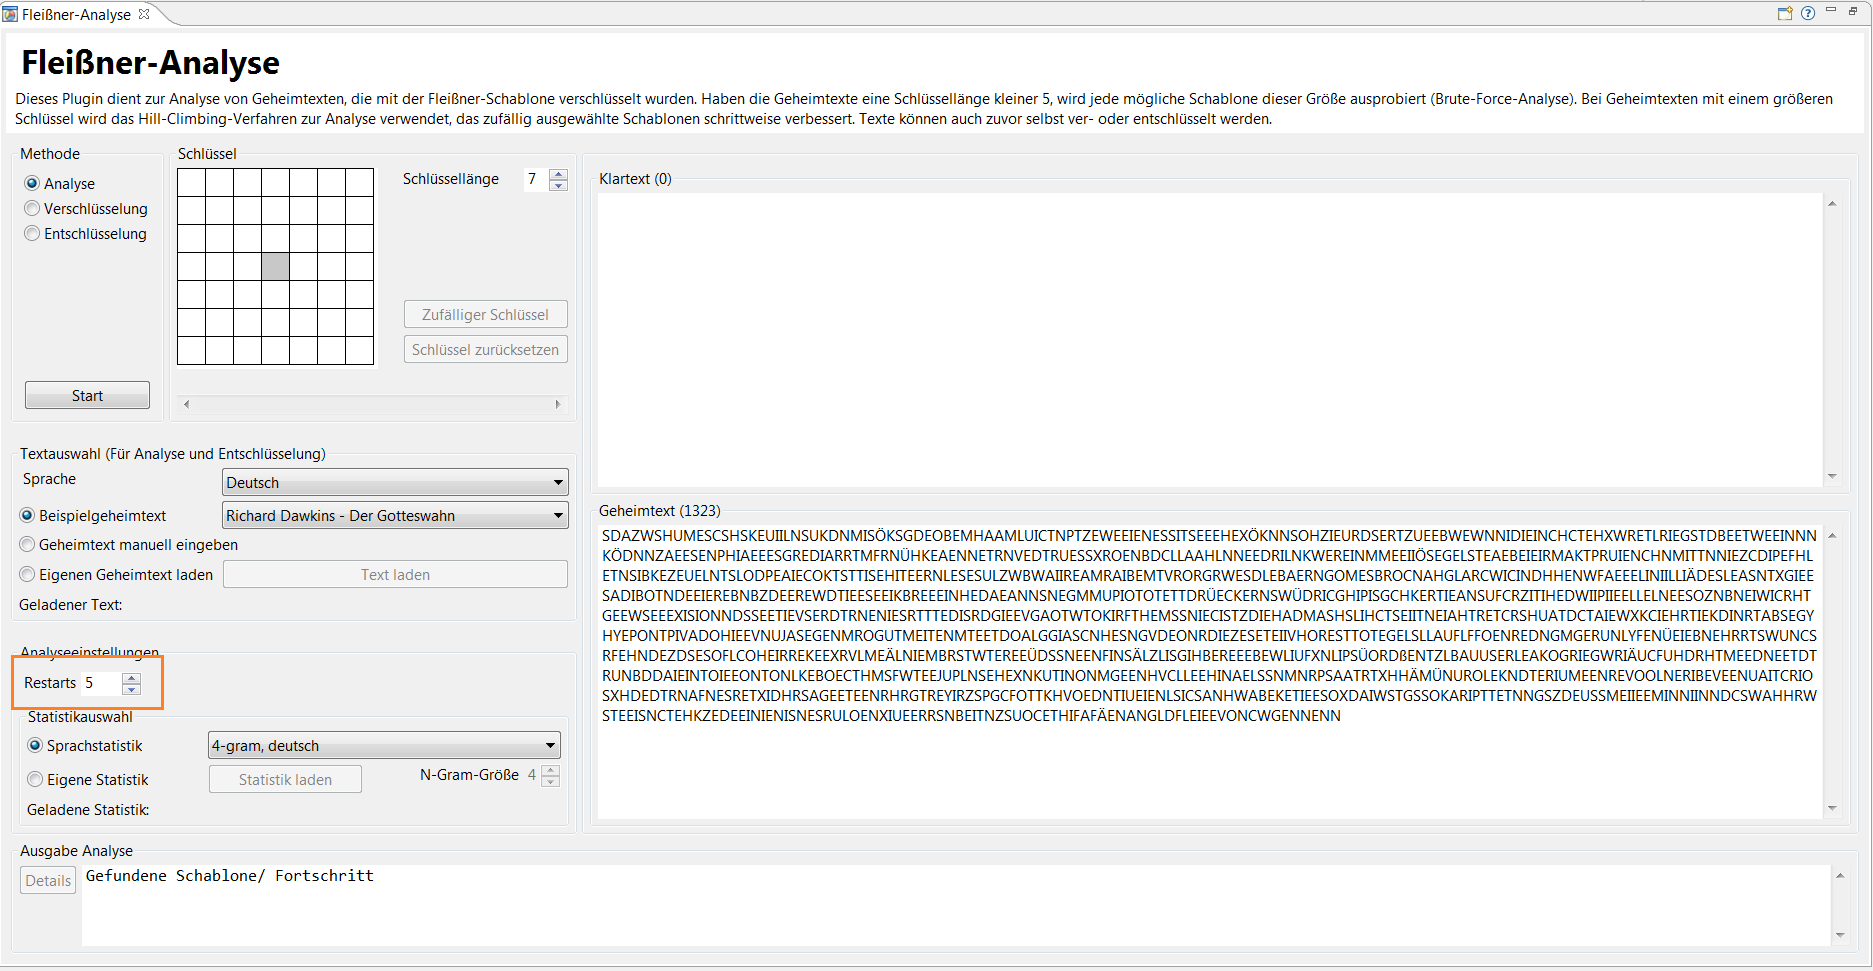
\includegraphics[scale=0.45]{FleissnerRestarts.png}

\textbf{Achtung:} Für große Schlüssel und eine hohe Restartanzahl ist mit einer langen Analysedauer zu rechnen. \footnote{Anhang: Evaluation der Analyse}

\subsubsection{Sprachstatistik}
Die Sprachstatistik ist essentiell für die Analyse eines Geheimtextes. In ihr sind die Auftrittswahrscheinlichkeiten aller zusammenhängenden Zeichenketten einer bestimmten Länge $n$ (n-Gramme) in der jeweiligen Sprache angegeben. Die Sprache des Geheimtextes muss mit der ausgewählten oder geladenen Statistik übereinstimmen, sonst sinkt die Erfolgswahrscheinlichkeit erheblich.

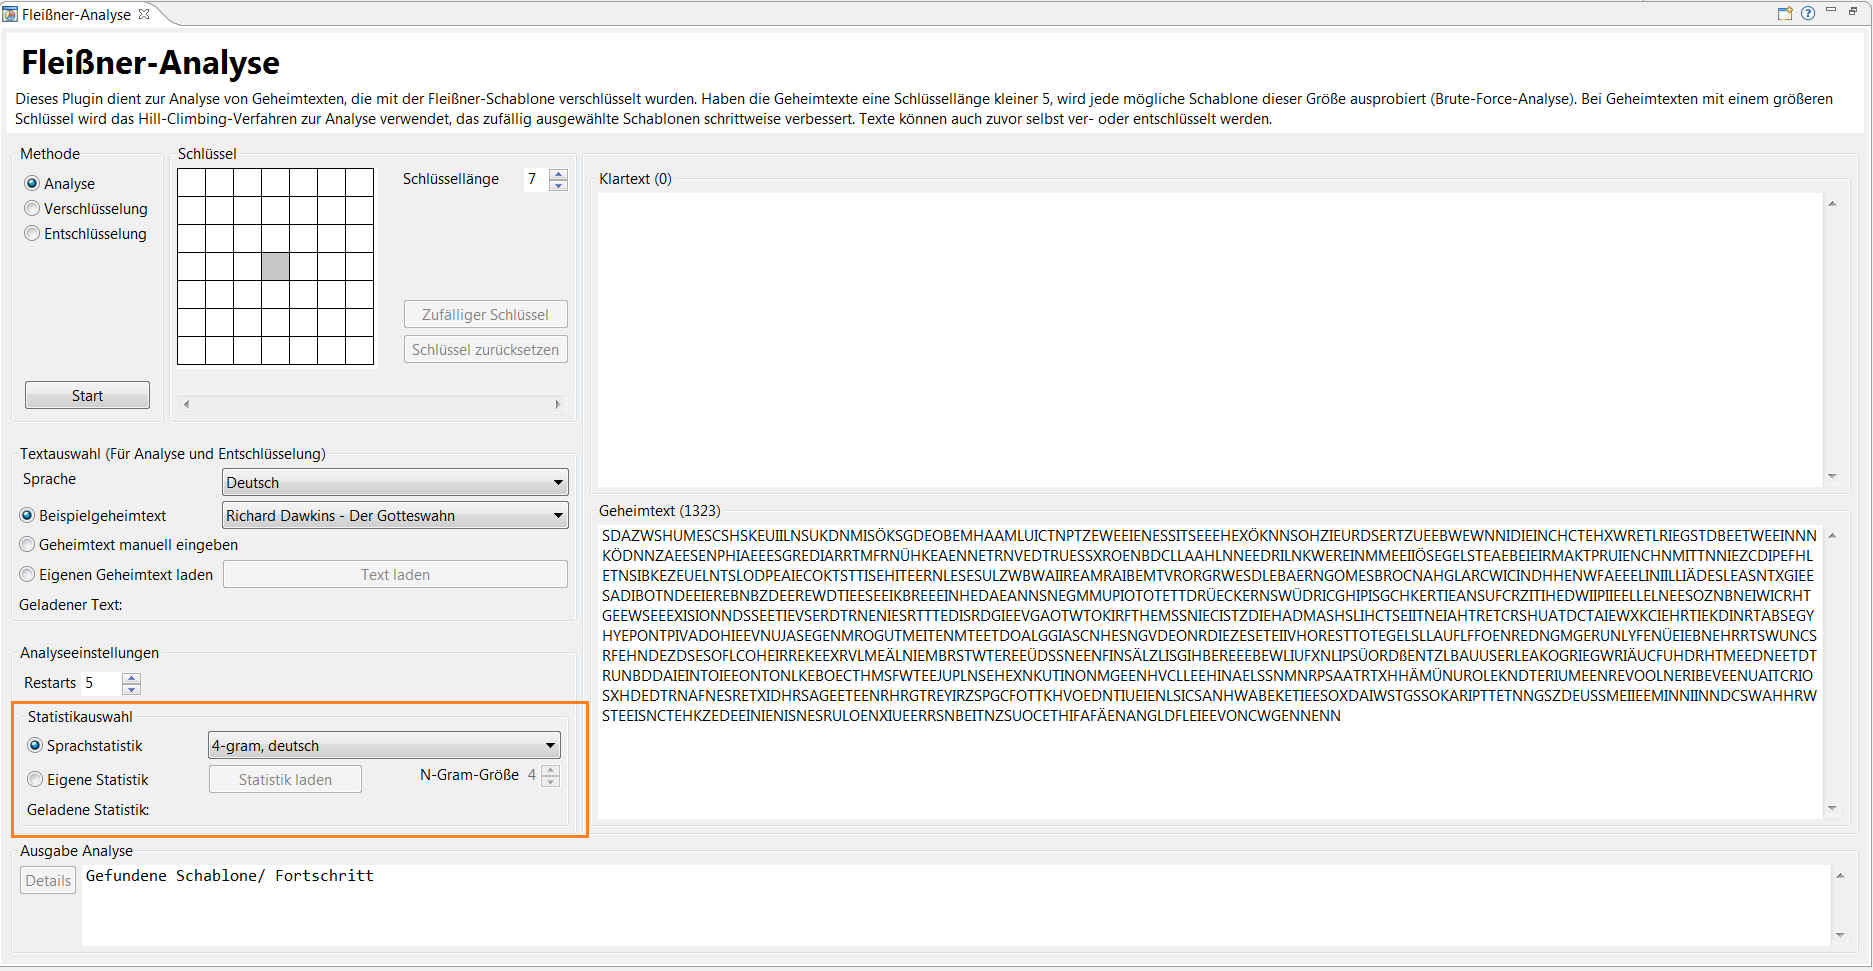
\includegraphics[scale=0.45]{FleissnerStatistics.png}

\begin{enumerate}[label=(\alph*), leftmargin=*]
\item \textbf{Sprachstatistik}

Zur Ausführung der Analyse kann eine der drei hinterlegten Statistiken genutzt werden. 

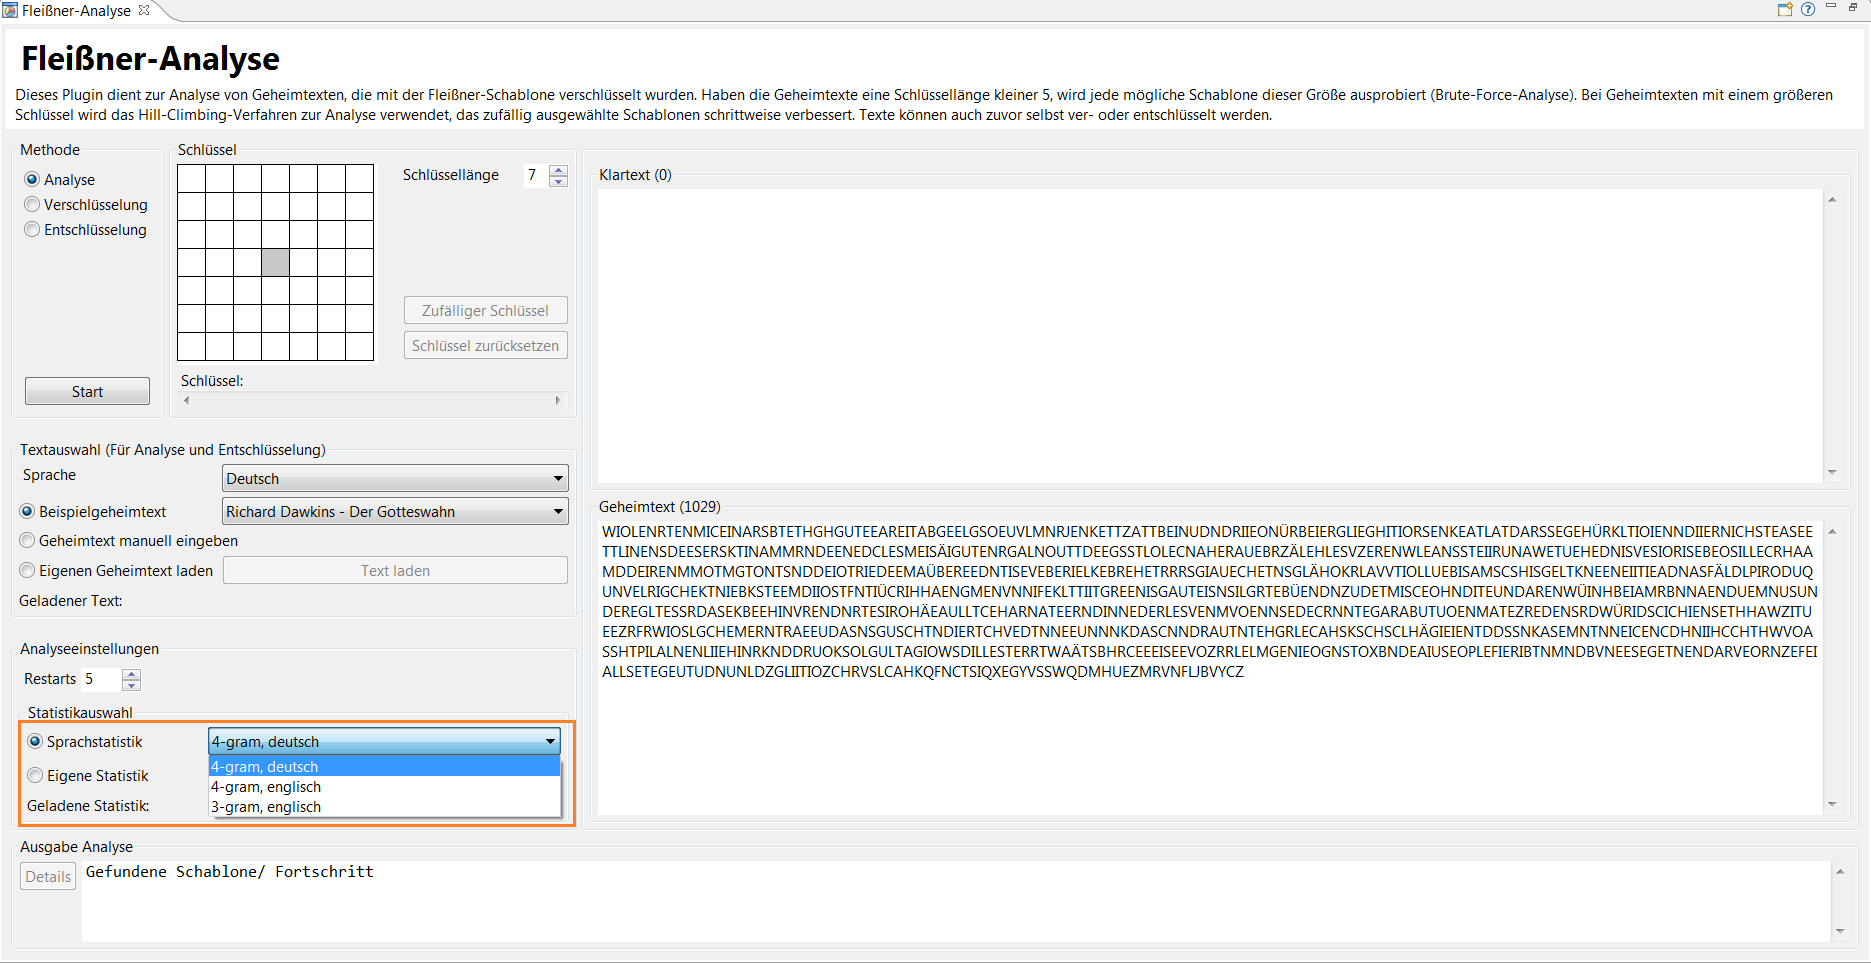
\includegraphics[scale=0.4]{FleissnerStatisticsExample.png}

\item \textbf{Eigene Statistik}

Es kann aber auch eine eigene Sprachstatistik-Datei geladen werden. Hierzu gelten gewisse \textit{Anforderungen} an das Format der Sprachstatistik:
Im Vergleich zu anderen Sprachstatistiken, sollten sich für dieses Plug-in die tatsächlichen n-Gramme nicht in der Datei befinden. Die genutzte Sprachstatistik sollte nur die bereits logarithmisierten Werte der jeweiligen n-Gramme enthalten. Dazu wird die Sprachstatistik wie ein $n$-dimensionaler Würfel aufgebaut, wobei die Position der Buchstaben im Alphabet sowie die Position jedes Buchstaben im n-Gramm gemeinsam den Index für den Wert zum jeweiligen n-Gramm angeben.

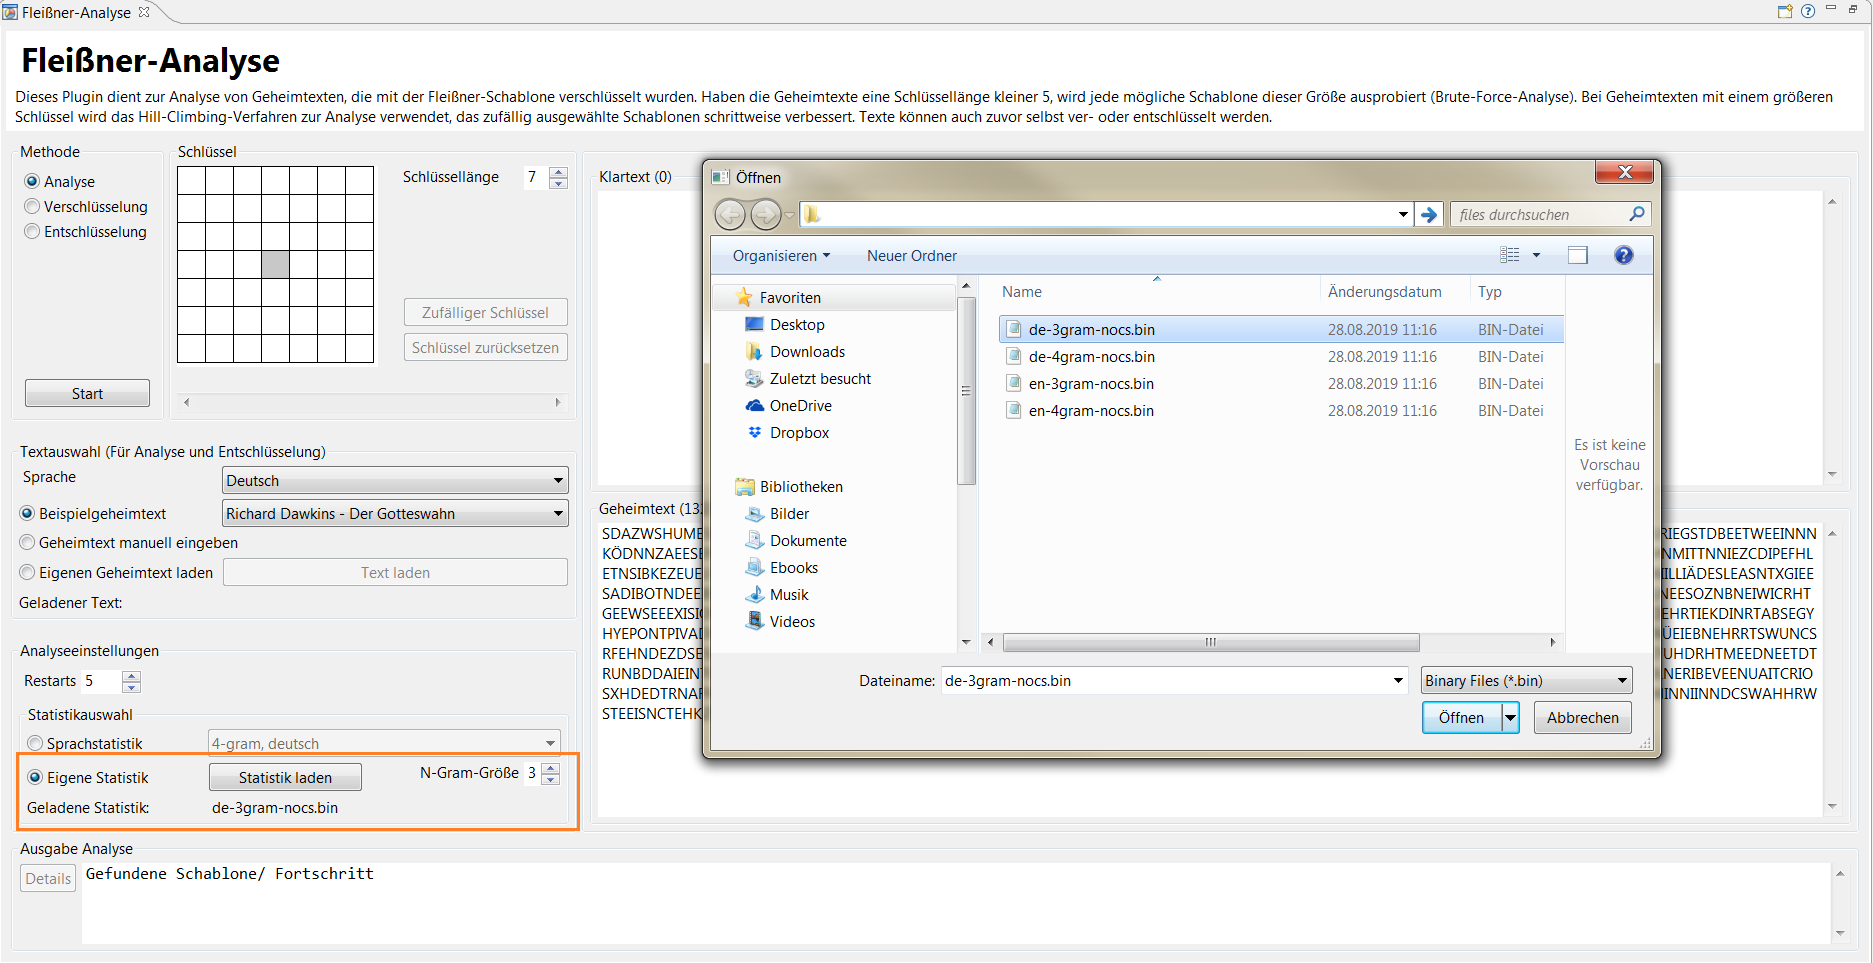
\includegraphics[scale=0.4]{FleissnerOwnStatistics.png}

\textbf{Beispiel:}
Zum Speichern und Abrufen des Quadgramms \glqq Ihre\grqq{} in einer deutschen Quadgramm-Statistik geht man wie folgt vor (wobei Kleinbuchstaben wie Großbuchstaben behandelt werden):

Das deutsche Alphabet wird mit angehängten Umlauten in einer Länge von 30 in der Form \glqq ABC...XYZÄÖÜß\grqq{} angegeben, wobei jedem Buchstaben ein Index von $0$ bis $29$ zugeordnet wird. Für das Quadgramm \glqq Ihre\grqq{} wird nun jeder Buchstabenindex des Quadgramms mit einer Potenz der Alphabetlänge in Abhängigkeit der Position im Quadgram multipliziert. Diese vier Werte werden addiert und ergeben zusammen den Index des Quadgrammwerts in der Sprachstatistik. So wie gerade erläutert, wird den Buchstaben I, h, r und e jeweils der Index 8, 7, 17 und 4 zugeordnet. Man berechnet nun

\[ 
8*30^3 + 7*30^2 + 17* 30^1+4*30^0 = 222.814
\]
für den Index des Quadgramms \glqq Ihre\grqq{} in einer deutschen Quadgramm-Statistik.

Wird eine eigene Sprachstatistik geladen, so muss hier in der Gruppierung \glqq Statistikauswahl\grqq{} zusätzlich die Größe der n-Gramme noch manuell angegeben werden.
\end{enumerate}
\newpage

\subsection{Ausgabe der Analyse}

Am unteren Bildschirmrand befindet sich das Ausgabefenster zur Analyse.
Hier werden zu Beginn der Analyse die ausgewählten Parameter angezeigt. Nach Abschluss der Analyse werden zusätzlich zur gefundenen Schablone der dadurch erzeugte Klartext sowie die benötigte Zeit hinzugefügt.

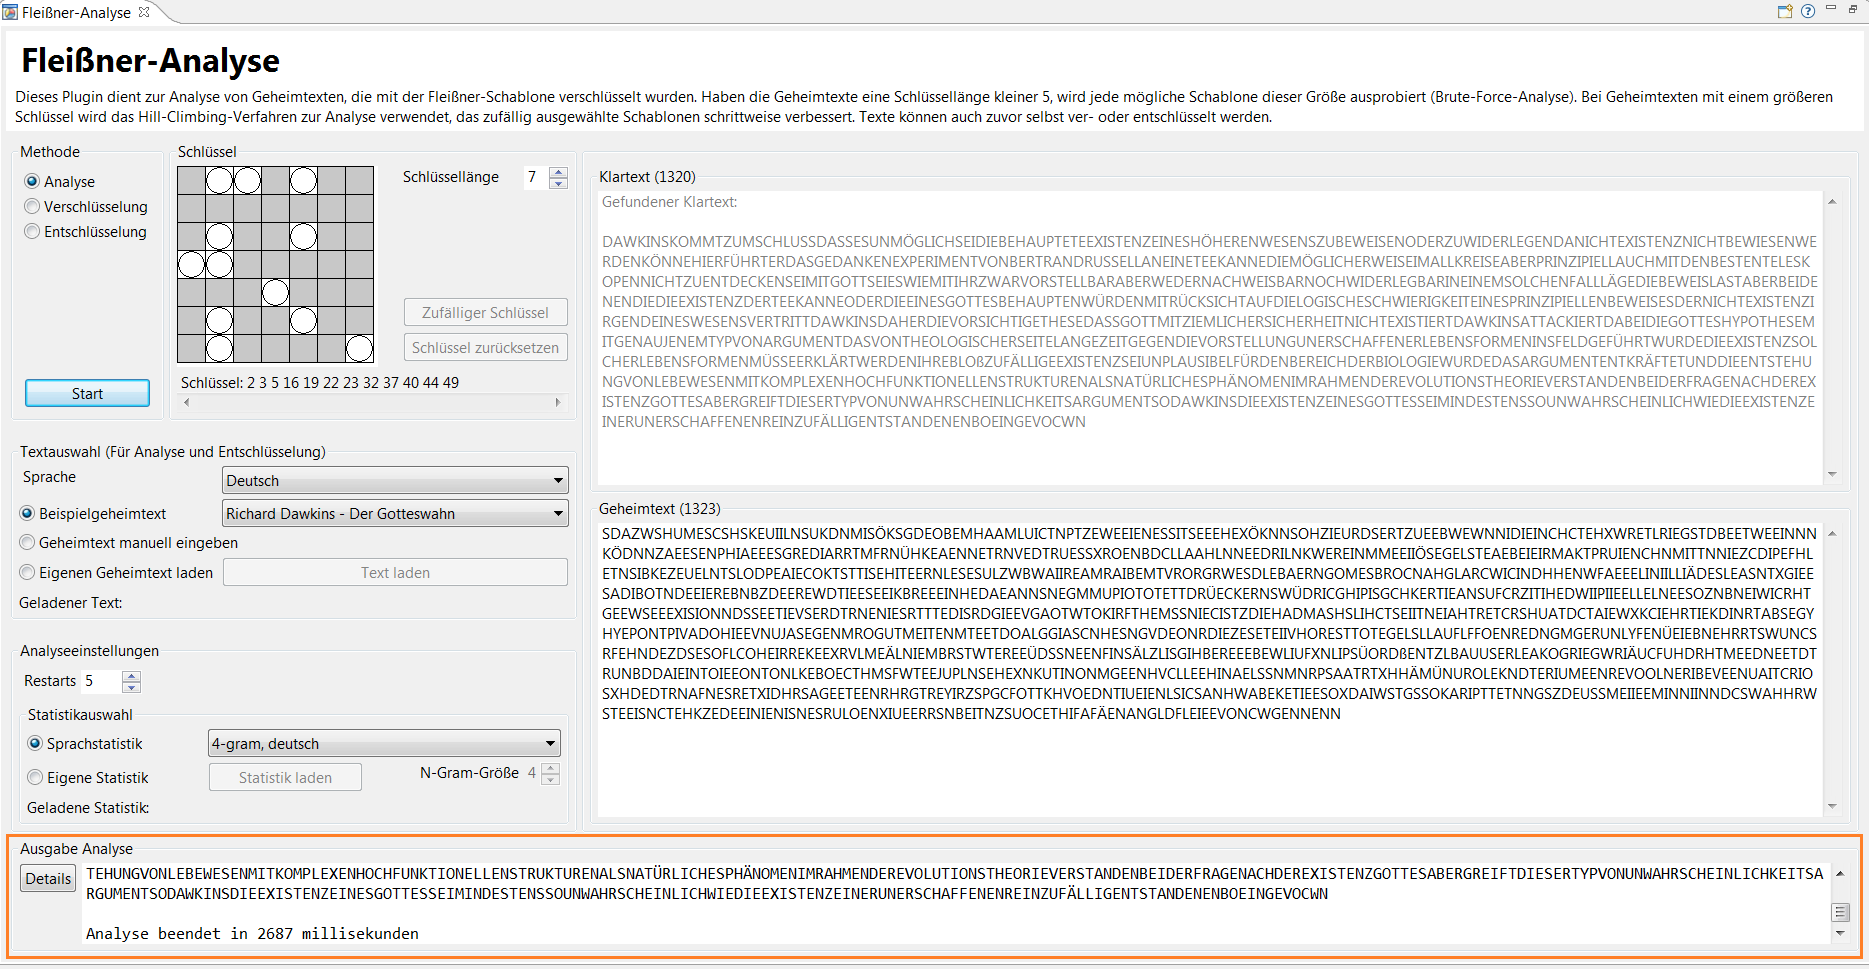
\includegraphics[scale=0.45]{FleissnerAusgabeAnalyse.png}

Für mehr Informationen befindet sich auf der linken Seite des Ausgabefelds der Button \glqq Details\grqq. 

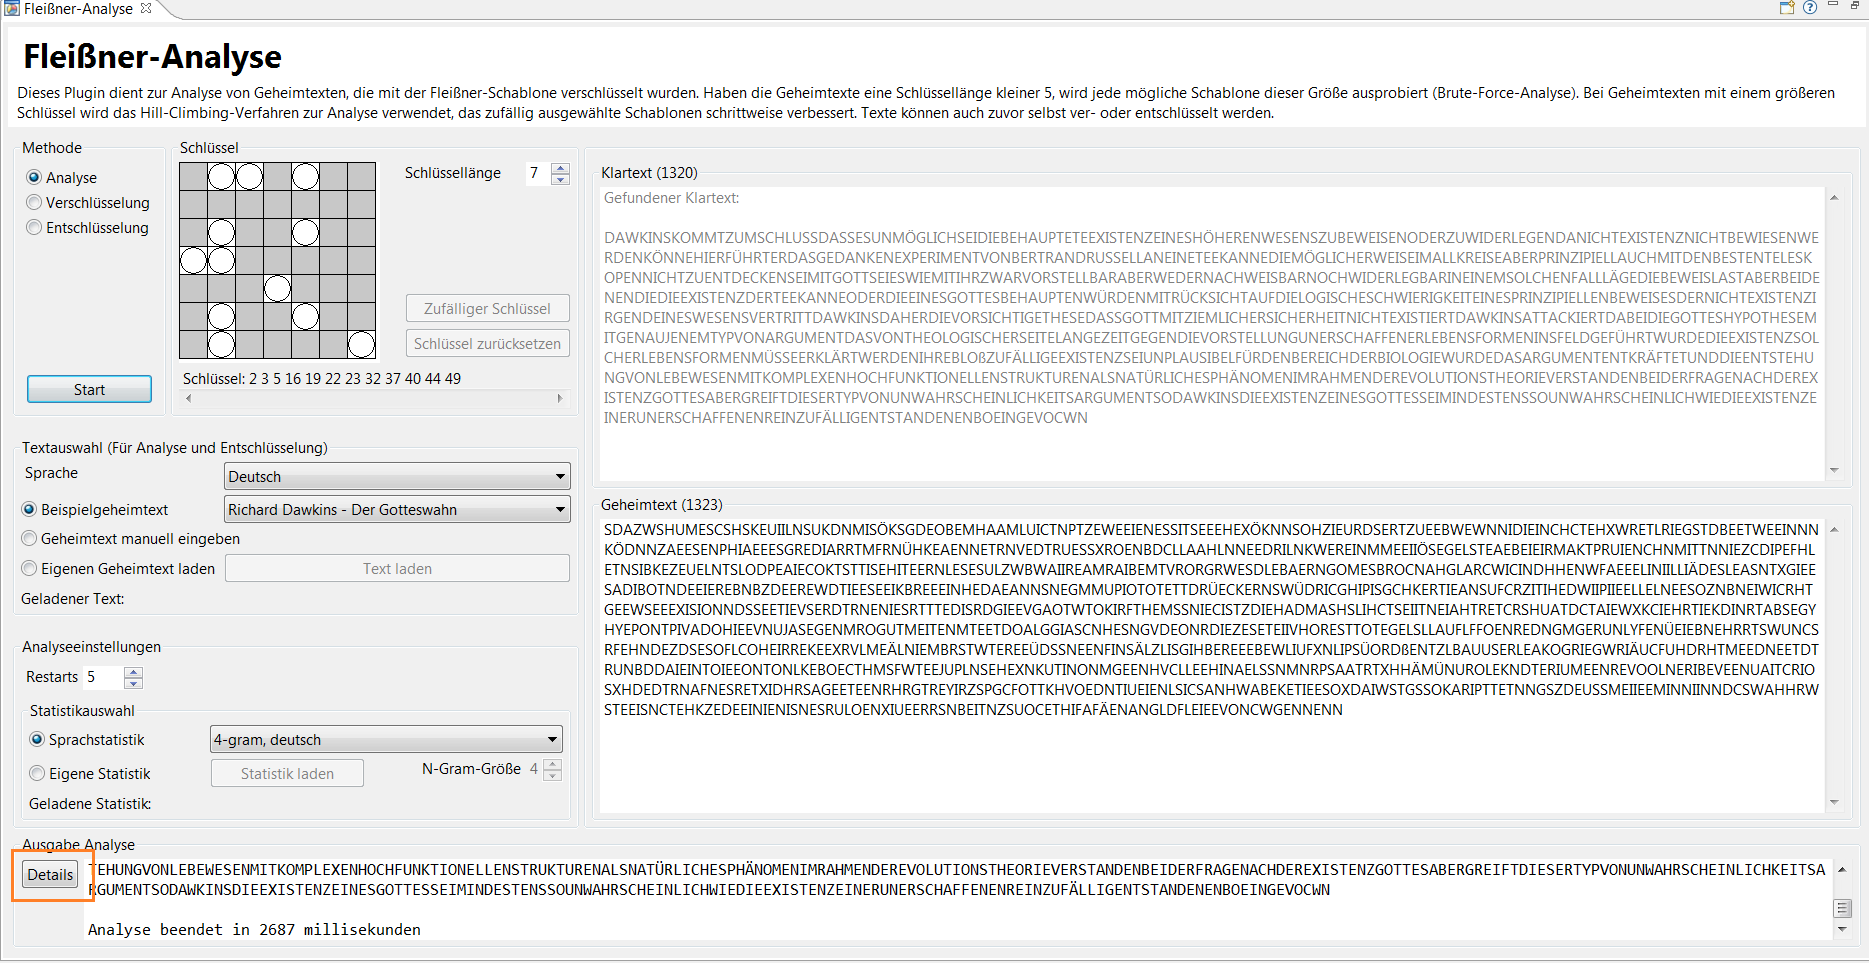
\includegraphics[scale=0.45]{FleissnerAusgabeAnalyseDetailButton.png}

Damit öffnet sich ein neues Dialogfenster, in dem zusätzlich zu den Informationen aus dem Ausgabefenster auch Zwischenausgaben aus dem Analyseprozess angezeigt werden. Diese Ausgabe kann dann auch als Textdatei (*.txt) gespeichert werden.

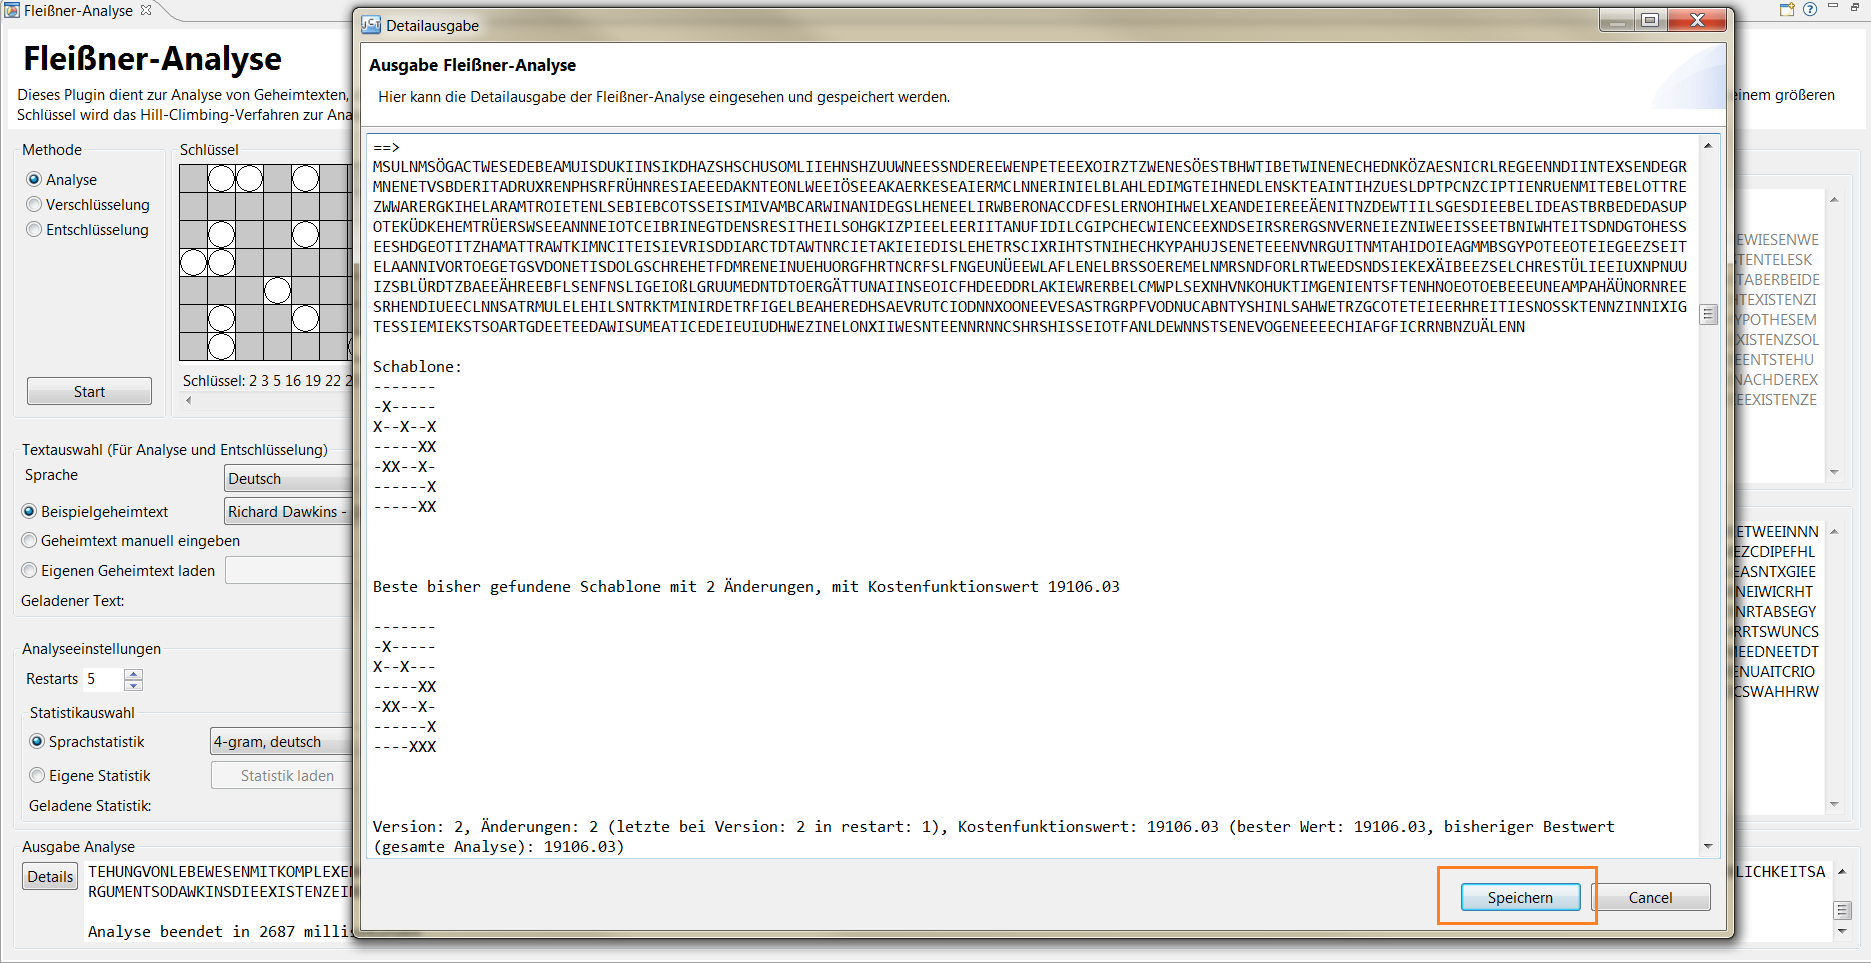
\includegraphics[scale=0.45]{FleissnerAusgabeAnalyseGross.png}

Nach Abschluss der Analyse wird der gefundene Schlüssel auch im Schlüsselfeld selbst angezeigt, so dass dieser beispielsweise direkt zur Entschlüsselung und damit Validierung des Analyseergebnisses verwendet werden kann.
\newpage

\section{Verschlüsselung}\hypertarget{verschl}{}
In diesem Plug-in können Klartexte auch selbst verschlüsselt werden. Dazu wird in der Gruppierung
\glqq Methode\grqq{} die Funktion \glqq Verschlüsselung\grqq{} ausgewählt. Dies aktiviert auch die Buttons zum Schlüssel-Erzeugen und -Zurücksetzen (ist Analyse ausgewählt, sind diese beiden Buttons deaktiviert).
 

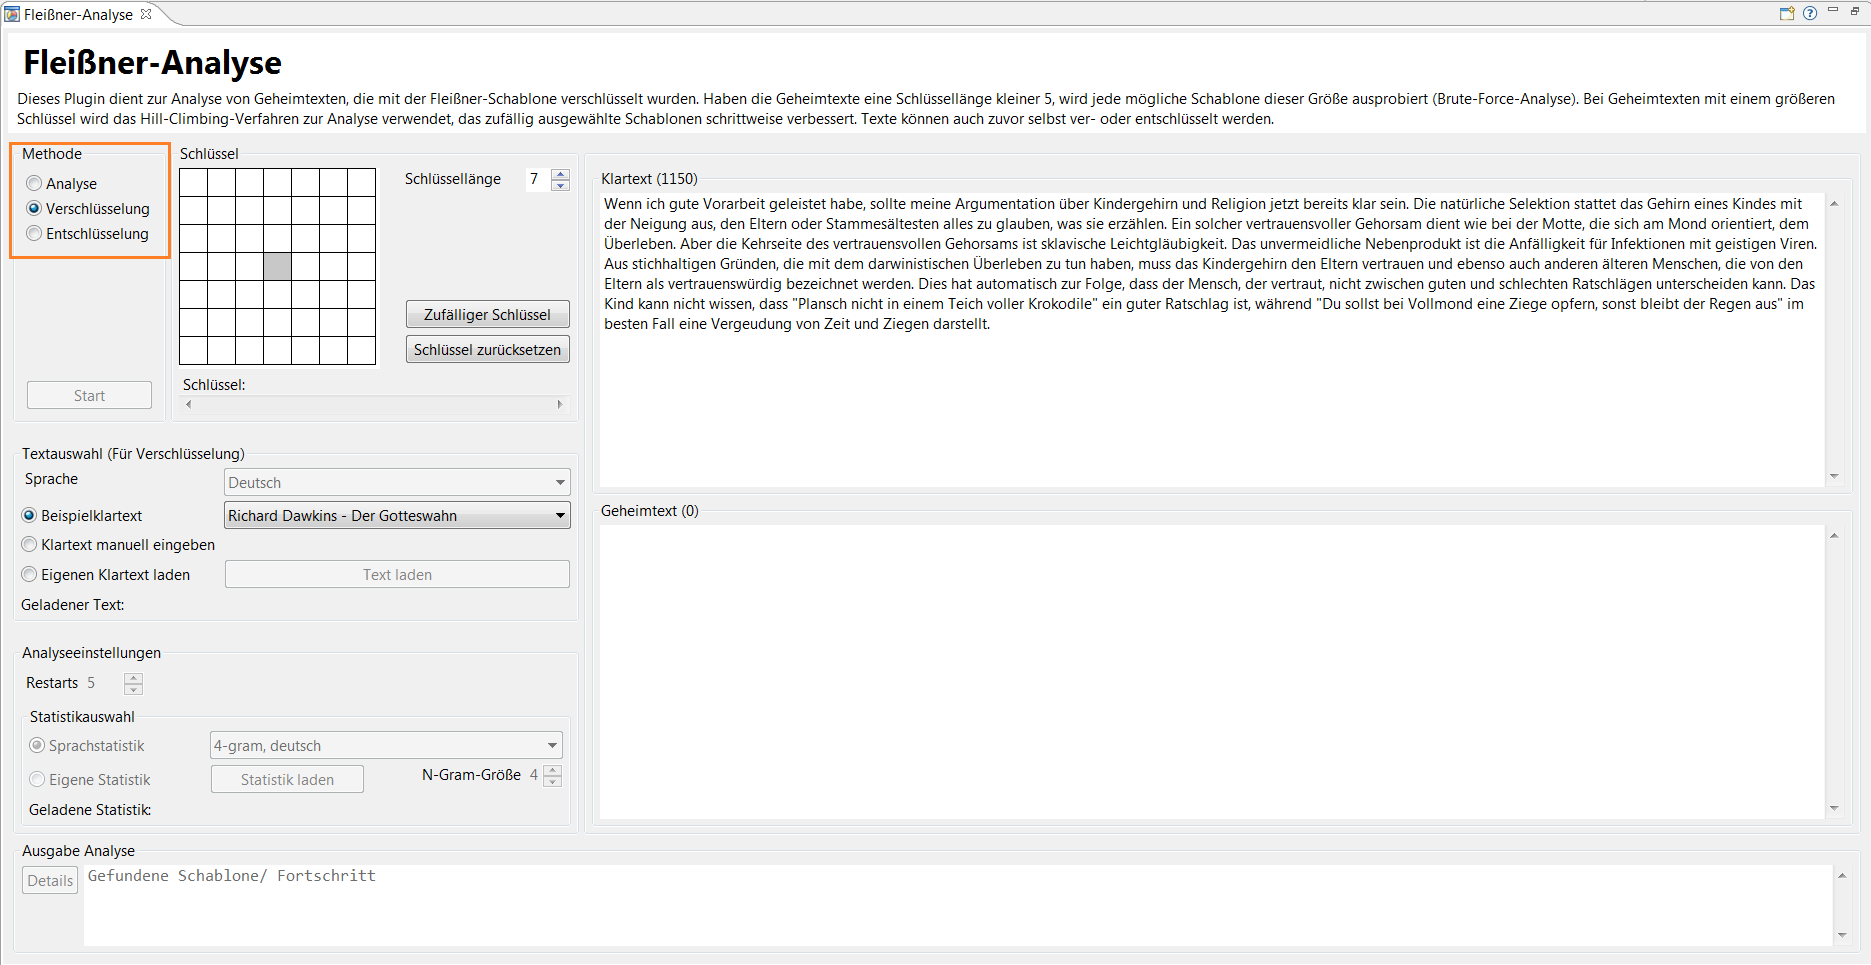
\includegraphics[scale=0.45]{FleissnerEncryptSelection.png}



\begin{enumerate}[label=(\alph*), leftmargin=*]
\item \textbf{Zufälliger Schlüssel}

Durch die Betätigung des Buttons \glqq Zufälliger Schlüssel\grqq{} wird ein zufälliger Schlüssel erzeugt und angezeigt. 

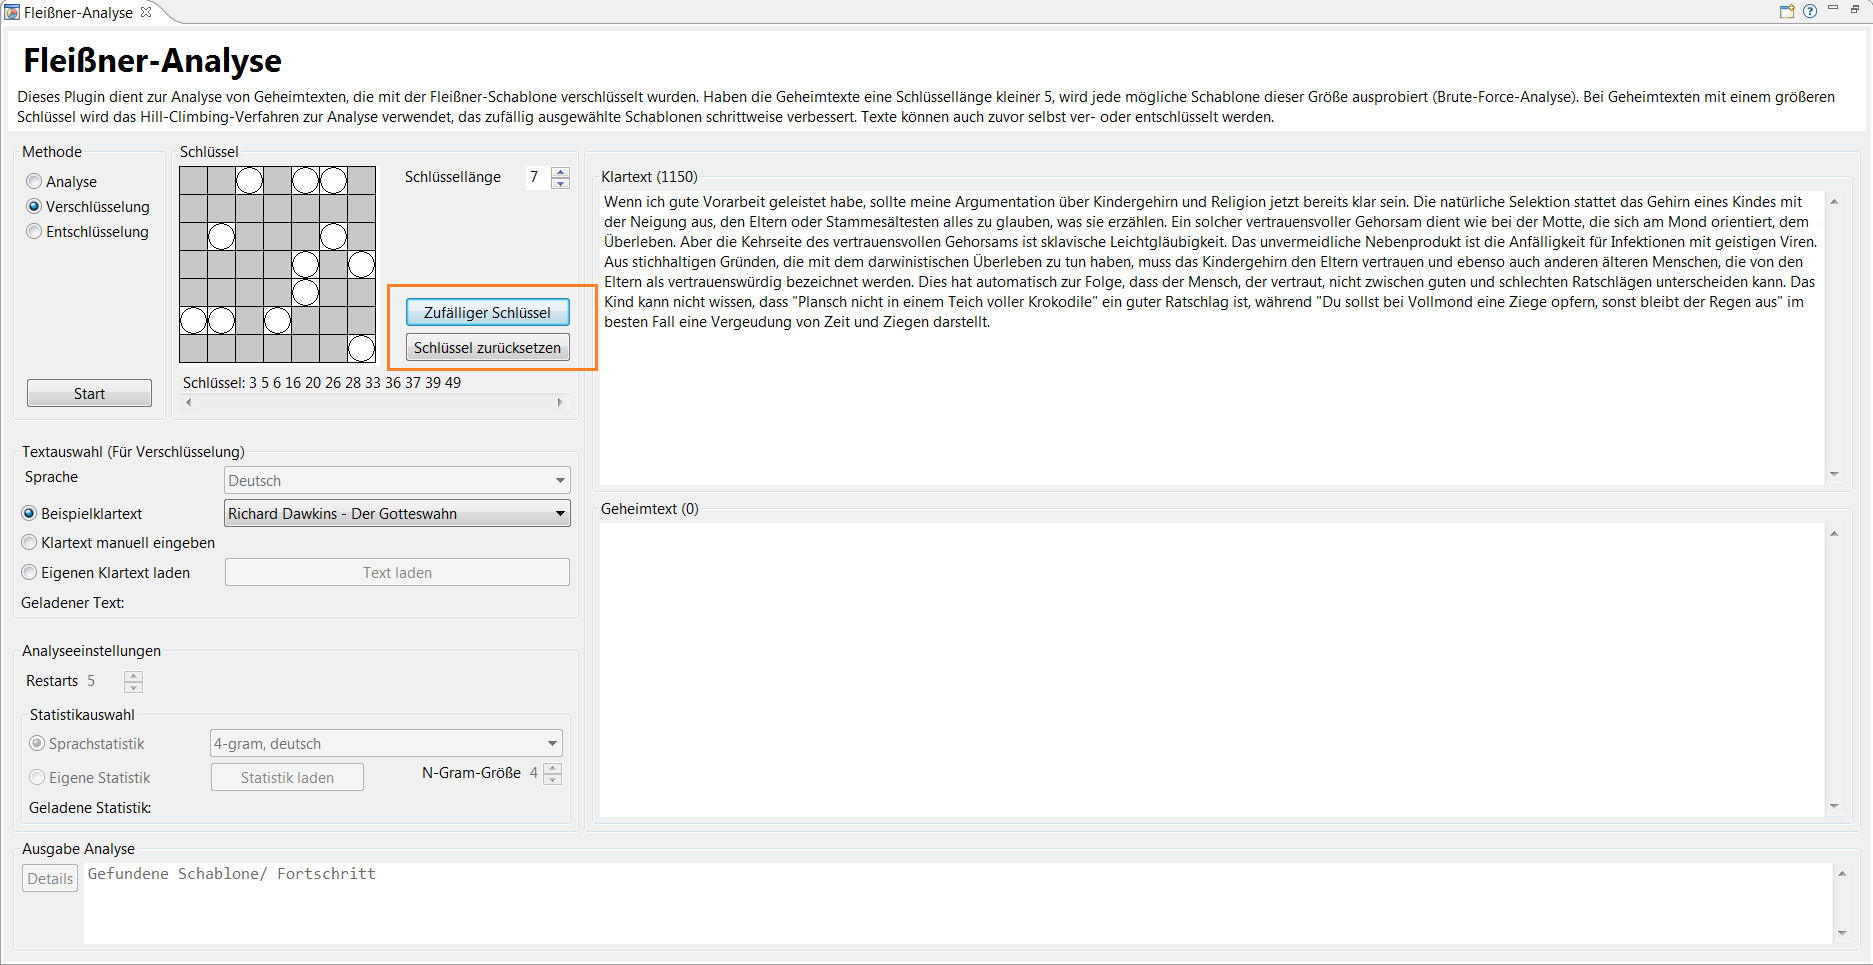
\includegraphics[scale=0.4]{FleissnerEncryptRandomKey.png}

\item \textbf{Manuelle Erstellung eines Schlüssels}

Für die manuelle Erstellung eines Schlüssel wählt man die Felder aus, an denen die Schablone die Löcher zum Eintragen des Klartextes enthalten soll. Für jedes ausgewählte Feld werden zugleich in den anderen 3 Quadranten die drei zugehörigen Felder blockiert, die durch die Rotation im Verschlüsselungsprozess benötigt werden. Wird ein bereits ausgewähltes Feld noch einmal angeklickt, so wird die Auswahl dieses Feldes rückgängig gemacht. 

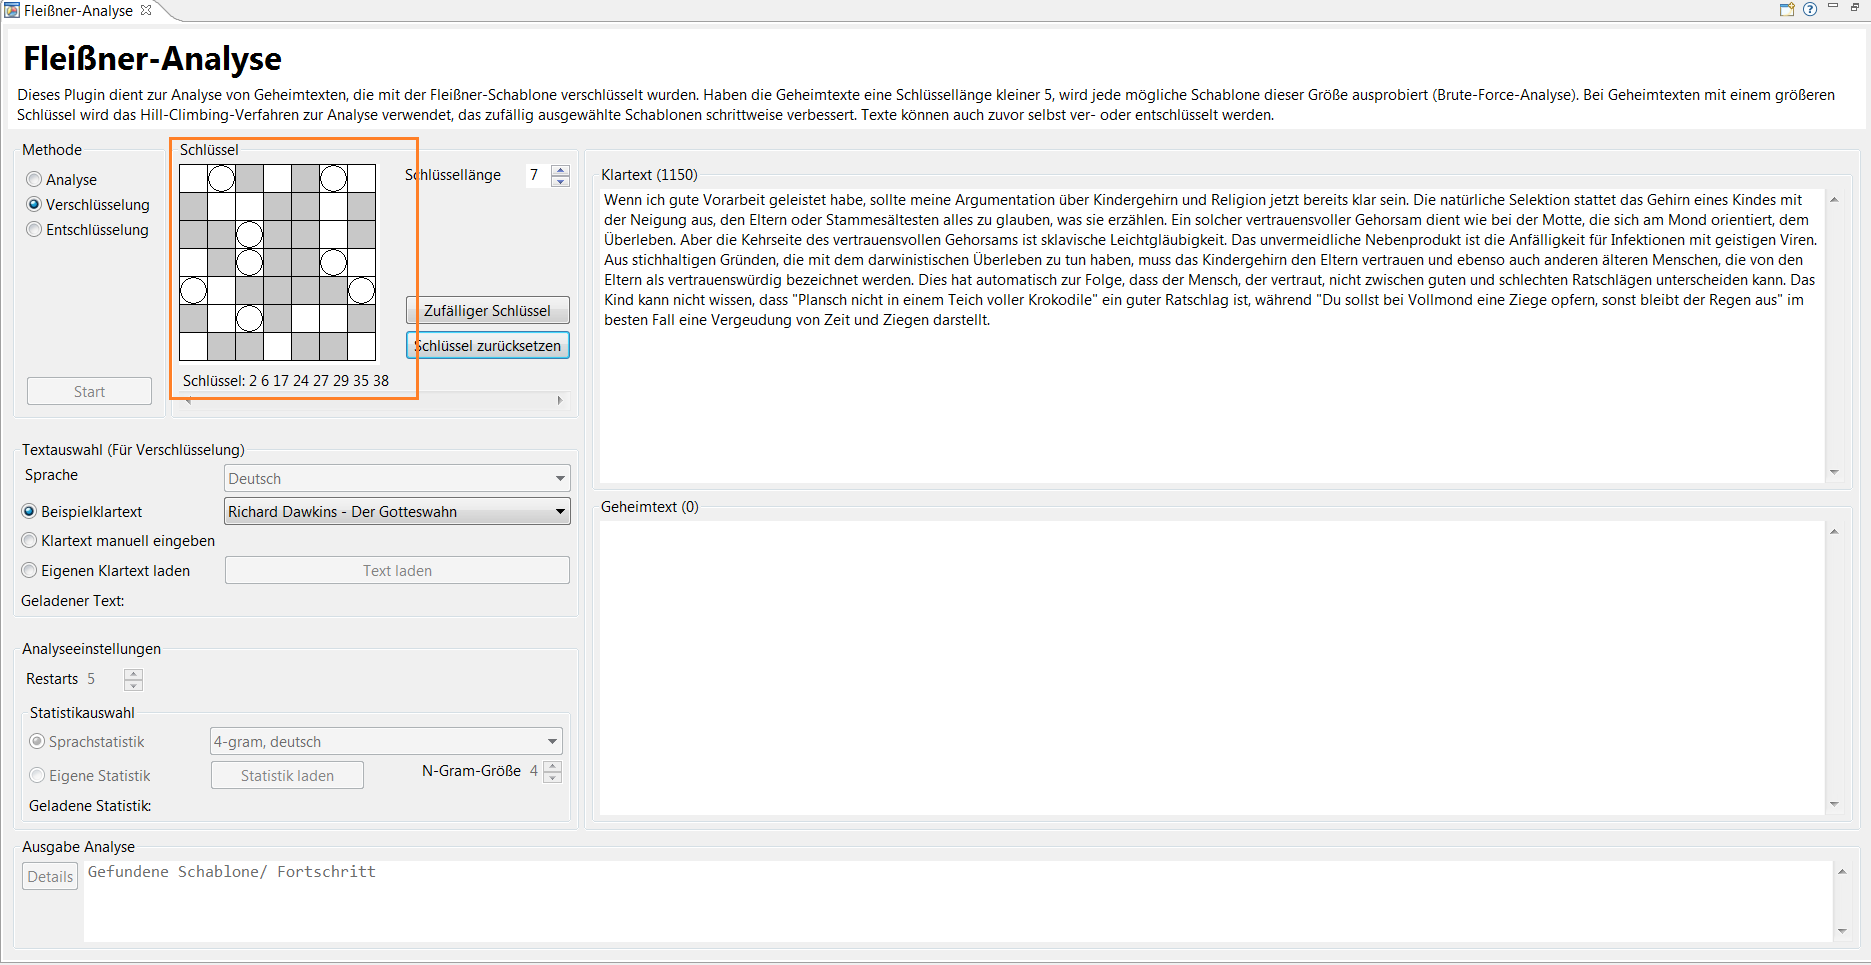
\includegraphics[scale=0.4]{FleissnerEncryptKeySelection.png}
\end{enumerate} 

Um die Auswahl aller Felder rückgängig zu machen, drückt man den \glqq Schlüssel zurücksetzen\grqq -Button.

Die ausgewählten Löcher des Schlüssels werden auch in Zahlenform unter dem Schlüsselfeld angezeigt. Die Felder sind hierzu von oben links nach unten rechts nummeriert (beginnend mit 1).


Zur Verschlüsselung ist neben dem Schlüssel auch ein Klartext erforderlich. Dieser kann wie auch in der Analysefunktion aus einer Menge von Beispieltexten gewählt, selbst eingetippt oder geladen werden. Bei der Auswahl von Beispieltexten wird die ausgewählte Funktion des Plug-ins erkannt und dementsprechend ein Klar- oder Geheimtext in das entsprechende Fenster geladen. Bei eigenen Texten muss diese Unterscheidung selbst getroffen werden. Das Plug-in erkennt bei selbst geladenen Texten nicht, ob ein Klartext oder ein Geheimtext vorliegt.

Liegt ein gültiger Schlüssel sowie ein Text im Klartextfeld vor, wird der \glqq Start\grqq -Button aktiviert und die Verschlüsselung kann durchgeführt werden. 

Nach Änderung der Methodenwahl auf \glqq Analyse\grqq{} oder \glqq Entschlüsselung\grqq{} kann mit dem selbst erzeugten Geheimtext fortgefahren werden.

\section{Entschlüsselung}\hypertarget{entschl}{}

Als letzte Funktionalität bietet das Plug-in eine Entschlüsselung an. Diese kann beispielsweise genutzt werden, um einen aus einer Analyse erhaltenen Schlüssel anzuwenden, aber auch um eigene Geheimtexte zu entschlüsseln. 

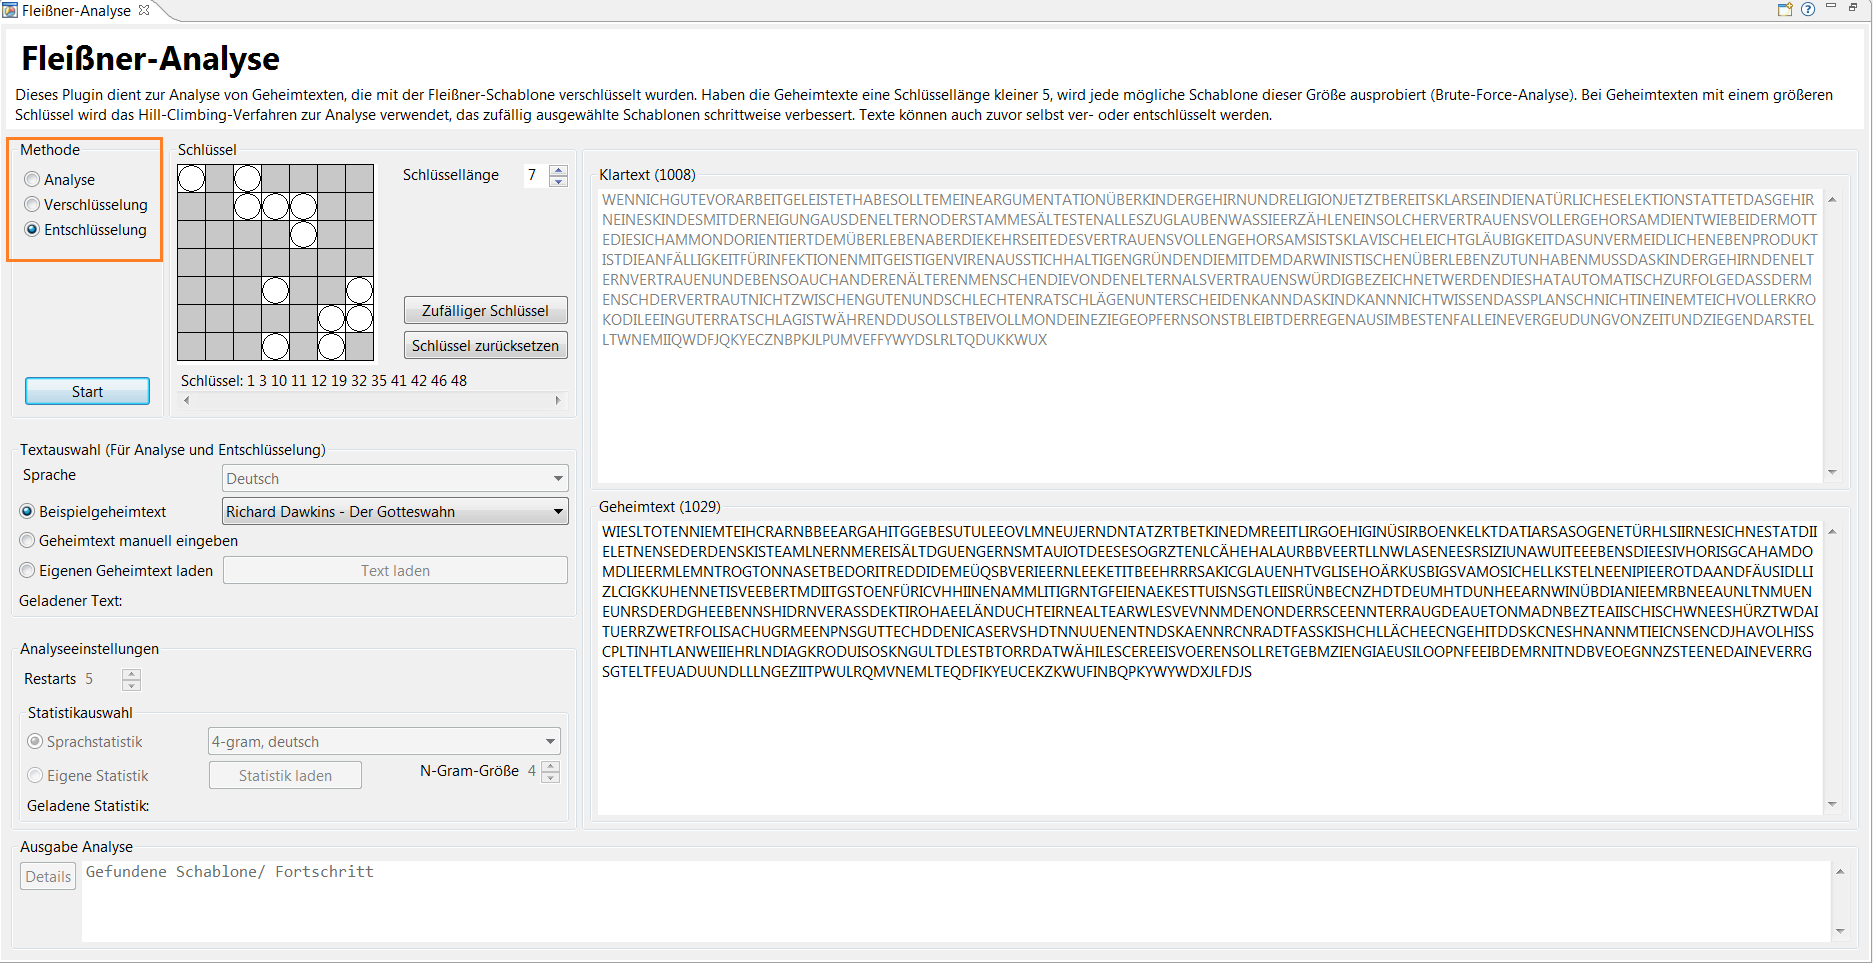
\includegraphics[scale=0.45]{FleissnerDecrypt.png}

Für die Entschlüsselung sowie auch schon für die Verschlüsselung wird ein gültiger Schlüssel und ein nichtleeres Geheimtextfeld benötigt. Die Bedienung der Textauswahl ist hier analog zu den beiden bereits beschriebenen Methoden.
\end{document}